\section{Präsentation der Ergebnisse}
\label{sec:PräsentationDerErgebnisse}

\subsection{Ergebnisdarstellung der Schülerumfrage}
\label{sec:ErgebnisdarstellungDerSchülerumfrage}

Die im folgenden Abschnitt dargelegten Ergebnisse spiegeln die Angaben der Schüler wieder, welche den Fragebogen korrekt ausgefüllt haben (154 von 175). Die implizierten Abbildungen beruhen auf der Datengrundlage von LimeSurvey, der Umfragesoftare welche zur Erstellung und Auswertung der Schülerumfrage herangezogen wurde.\\

\noindent
Es wird darauf hingewiesen, das die Legendenbeschriftung der Abbildungen aufgrund der Lesbarkeit sinnvoll eingekürzt wurde. Die Originalbeschriftung der Abbildungen sind der LimeSurvey-Statistik (Punkt \ref{sec:Ergebnisauswertung}) bzw. der Schülerumfrage im Anhang zu entnehmen (Punkt \ref{sec:Schülerumfrage}).\\

\noindent
\textbf{Abschnitt 1: Allgemeine Angaben zur Person}\\

\noindent
Wie bereits dargelegt, sind die allgemeinen Angaben zur Person bei der Beantwortung der Forschungsfragen nicht zwingend von Belang. Dennoch sind sie von Interesse bei der späteren Interpretation der Ergebnisse da sie das Klientel der Berufsschüler in seiner Heterogenität verdeutlicht. Mögliche Probleme können so besser eingeordnet und Unterstützungsbedarfe besser auf die Grundgesamtheit abgestimmt werden.

An der Schülerumfrage am DRK Bildungswerk SN nahmen 154 Schüler teil. Es wurden dabei 111 weibliche und 43 männliche
Schüler befragt. Das entspricht einer weiblichen Mehrheit von $\approx$ 72\% zu $\approx$ 28\%. Die befragten Schüler wiesen eine Altersspanne von maximal 27 Jahren auf, d. h. die jüngsten Schüler entstammen dem Geburtsjahr 1998 und die "`ältesten"' Schüler entstammen dem Jahr 1971. Das durchschnittliche Geburtsjahr lässt sich auf das Jahr 1991 datieren. Die Frage nach dem Bildungsabschluss konnte mehrfach beantwortet werden wenn Schüler neben einem Schulabschluss bereits einen Berufsabschluss erlangt haben. Die bisherigen Bildungsabschlüsse stellen sich wie folgt dar (Abb.: \ref{fig:Hoechster-bisher-erreichter-Bildungsabschluss}):

\begin{figure}[ht]
	\centering
		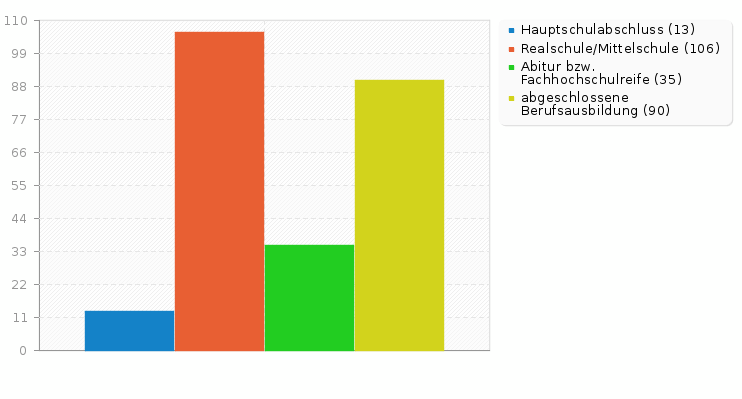
\includegraphics[width=1.0\textwidth]{images/Hoechster-bisher-erreichter-Bildungsabschluss.png}
	\caption{höchster bisher erreichter Bildungsabschluss}
	\label{fig:Hoechster-bisher-erreichter-Bildungsabschluss}
\end{figure}

\noindent
Wie der Abbildung zu entnehmen ist, besitzen 90 Schüler neben einem unterschiedlichen Schulabschluss, bereits einen weiterführenden Berufsabschluss. Die befragten Berufsschüler weisen somit mehrheitlich ($\approx$ 58,4\%) eine berufliche Vorbildung auf. Die spezifische Berufsbezeichnung wurde nicht erfragt.\\

\noindent
\textbf{Abschnitt 2: Ermittlung der persönlichen Problemlagen und Annahme außerunterrichtlicher Unterstützungsangebote}\\

\noindent
In diesem Abschnitt steht die persönliche Sichtweise der befragten Schüler im Fokus. 139 Personen ($\approx$ 90\%) gaben an, das sie im Laufe ihrer jetzigen Ausbildung schwierige Problemsituationen erlebt haben, welche sich in der Vergangenheit oder aktuell negativ auf die Ausbildung ausgewirkt haben bzw. auswirken. Nur 15 Personen gaben an, keine Probleme (gehabt) zu haben. 

Zu Visualisierung der Problemlagen wurden im Anschluss folgende Punkte von den 139 Personen benannt (Abb.: \ref{fig:Aktuelle-oder-vergangene-Probleme-der-Schueler-welche-die-Ausbildung-negativ-beeinflussen-oder-negativ-beeinflusst-haben}). Mehrfachnennungen waren hierbei möglich. 

\begin{figure}[ht]
	\centering
		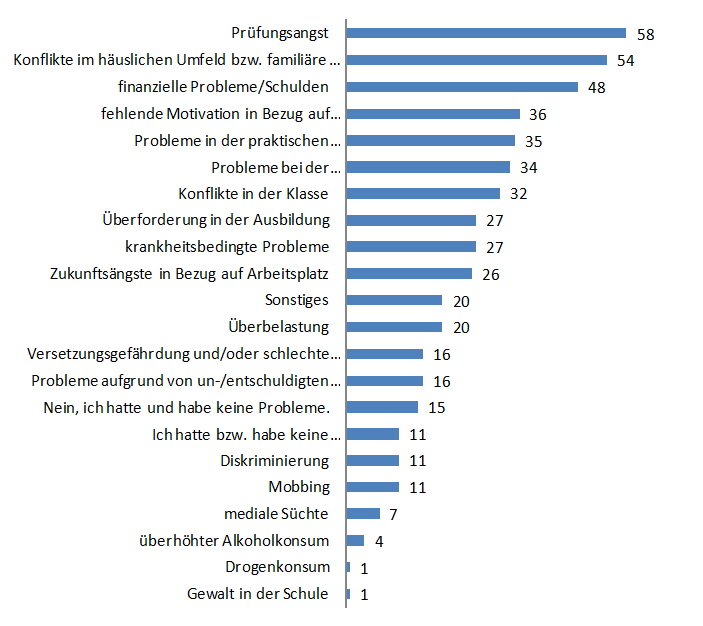
\includegraphics[width=1.0\textwidth]{images/Aktuelle-oder-vergangene-Probleme-der-Schueler-welche-die-Ausbildung-negativ-beeinflussen-oder-negativ-beeinflusst-haben.png}
	\caption{persönliche aktuelle oder vergangene Problemlagen, welche die Ausbildung negativ beeinflussen oder beeinflusst haben}
	\label{fig:Aktuelle-oder-vergangene-Probleme-der-Schueler-welche-die-Ausbildung-negativ-beeinflussen-oder-negativ-beeinflusst-haben}
\end{figure}

\noindent
Bei der mannigfaltigen Nennung an Problemlagen, heben sich Folgende verstärkt ab (ab 30 Nennungen!):

\begin{itemize}
	\item Prüfungsangst (58)
	\item Konflikte im häuslichen Umfeld bzw. familiäre Probleme (54)
	\item finanzielle Problem/Schulden (48)
	\item fehlende Motivation in Bezug auf Schule/Ausbildung (36)
	\item Probleme in der praktischen Ausbildung/Praktikum (35)
	\item Probleme bei der Wissensaneignung/fehlende Lernstrategien (34)
	\item Konflikte in der Klasse (32)
\end{itemize}

\noindent
Diese 7 Punkte repräsentieren einen großen Teil der Problemlagen der Schülerschaft am DRK Bildungswerk SN. Die restlichen 12 Probleme weisen jedoch ebenfalls vielfache Nennungen auf und sollten bei der komplexen Betrachtung der vorhandenen Problemlagen der Schüler berücksichtigt werden. Da es jedoch unrealistisch ist, anzunehmen das für alle Problemlagen passende Angebote am DRK Bildungswerk SN initiiert werden können, soll der Fokus der Betrachtung auf diese 7 Hauptprobleme gelegt werden.

Die Liste der Probleme konnte um individuell Angaben ergänzt werden, was von 18 Schüler in Anspruch genommen wurde. Dabei wurden Probleme wie Depressionen, Borderline-Erkrankung, Tod eines Familienmitgliedes, Zeitstress durch nebenberufliche Tätigkeit, Fehlgeburt(en) oder auch Versagensangst angesprochen. Da diese Problemlagen jedoch Einzelfälle darstellen, werden sie hier nicht näher betrachtet, auch wenn sie für den Einzelnen z. T. sehr belastend sind oder waren.

Wenn Personen von Problemen betroffen sind, wird häufig das Gespräch mit anderen Personen gesucht. Die Schüler gaben hierfür folgende Ansprechpartner an (Abb.: \ref{fig:welche-Personen-wurden-bisher bei-persoenlichen-Problemen-in-der-zurueckliegenden-Ausbildungszeit-fuer-Gespraeche-in-Anspruch-genommen}). Mehrfachnennungen waren möglich. 

\begin{figure}[ht]
	\centering
		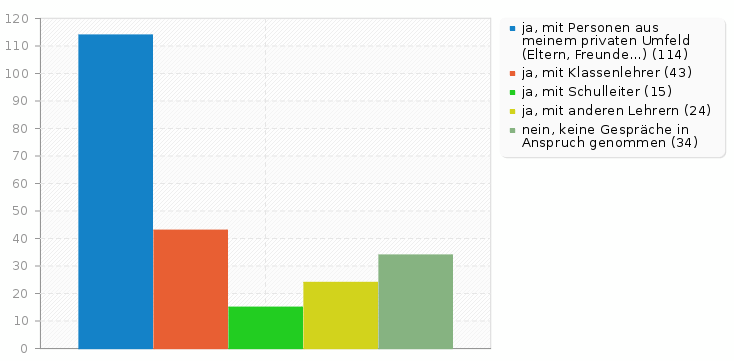
\includegraphics[width=1.0\textwidth]{images/welche-Personen-wurden-bisher-bei-persoenlichen-Problemen-in-der-zurueckliegenden-Ausbildungszeit-fuer-Gespraeche-in-Anspruch-genommen.png}
	\caption{Personen, welche bei persönlichen Problemen für Gespräche bisher in Anspruch genommen wurden}
	\label{fig:welche-Personen-wurden-bisher bei-persoenlichen-Problemen-in-der-zurueckliegenden-Ausbildungszeit-fuer-Gespraeche-in-Anspruch-genommen}
\end{figure}

\noindent
Diese Frage verdeutlicht, das ein Großteil der Befragten bei persönlichen Problemen zunächst Personen aus dem Familien- und Freundeskreis (114) zu Rate ziehen. Dennoch werden auch Lehrer (24) und Klassenlehrer (43) bei Problemen um ein Gespräch ersucht.

Das DRK Bildungswerk SN hat zum Zeitpunkt der Befragung einen Vertrauenslehrer. Auch diese Person kann bei Problemen um Rat gefragt werden. Jedoch geben nur 7 von 154 Schülern an, dieses Unterstützungsangebot in der bisherigen Ausbildungszeit genutzt zu haben. Die Gründe hierfür sind verschieden. 48 Personen wussten bspw. nicht das es einen Vertrauenslehrer an der Schule gibt, 21 Personen wussten bis dahin nicht wo und wann die betreffende Person zu erreichen ist und 104 Schüler konstatierten, dank der erlaubten Mehrfachnennung, das sie den Vertrauenslehrer bei persönlichen Problemen nicht aufsuchen würden. Explizite Gründe für eine Nichtinanspruchnahme des Vertrauenslehrers werden von 14 Schülern wie folgt aufgezeigt (Abb.: \ref{fig:Gruende-fuer-die-Nichtinaspruchnahme-des-Vertrauenslehrers}).

\begin{figure}[ht]
	\centering
		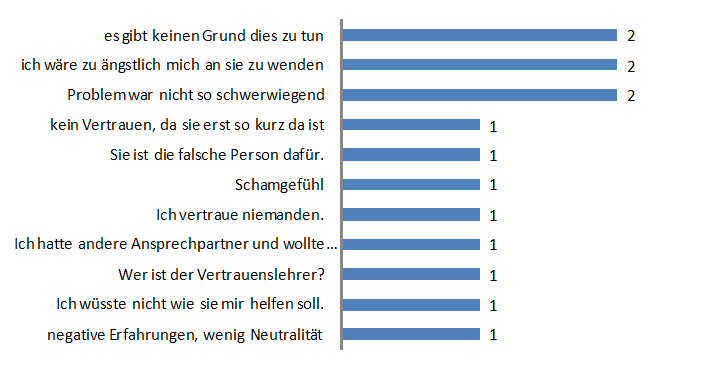
\includegraphics[width=1.0\textwidth]{images/Gruende-fuer-die-Nichtinaspruchnahme-des-Vertrauenslehrers.png}
	\caption{Gründe für die bisherige Nicht-Inanspruchnahme des Vertrauenslehrers am DRK Bildungswerk SN}
	\label{fig:Gruende-fuer-die-Nichtinaspruchnahme-des-Vertrauenslehrers}
\end{figure}

\noindent
Diese individuellen Gründe der Nicht-Inanspruchnahme des Vertrauenslehrers, werden bei der Interpretation der Ergebnisse und in der Konzeption möglicher Beratungs- und Unterstützungsangebote erneut aufgegriffen. Besonders die Aspekte Angst, fehlendes Vertrauen und Schamgefühl gilt es hierbei zu beachten. 

Die letzten 3 Fragen von Abschnitt 2 betrachten das potentielle Angebot weiterführender Beratungs- und Unterstützungsangebote. 

56 von 154 befragten Schülern könnten sich vorstellen außerunterrichtliche Beratungs- und Unterstützungsangebote in der Schule in Anspruch zu nehmen. Im Gegensatz dazu würden 98 Schüler ($\approx$ 63,6\%) keine Angebote in Anspruch nehmen, wobei 16 von 98 ihre Entscheidung begründeten. Die angegebenen Gründe reichen von "`keine  zeit"' (4), "`kein Vertrauen"' (2), über eine klare Abgrenzung von Privaten und Beruflichen (2) bis hin zur Ablehnung von Hilfeleistungen durch das DRK Bildungswerk SN (1). Diese Angaben gilt es bei der Konzeption möglicher Beratungs- und Unterstützungsangebote zu berücksichtigen, auch wenn sie nur einen Teil der Schülerschaft repräsentieren.

Zuletzt wurde der Personenkreis von denen Beratungs- und Unterstützungsangebote angenommen werden würde (Abb.: \ref{fig:Von-welchen-Personen-wuerden-unterstuetzende-Angebote-angenommen}), sowie Rahmenbedingungen dieser Angebote erfragt (Abb.: \ref{fig:Rahmenbedingungen-fuer-Unterstuetzungangebote}). 

\begin{figure}[ht]
	\centering
		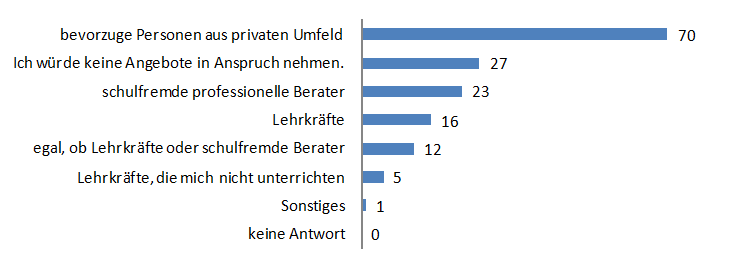
\includegraphics[width=1.0\textwidth]{images/Von-welchen-Personen-wuerden-unterstuetzende-Angebote-angenommen.png}
	\caption{Personen, von denen Angebote in Anspruch genommen werden würden}
	\label{fig:Von-welchen-Personen-wuerden-unterstuetzende-Angebote-angenommen}
\end{figure}

\noindent
Die 56 Personen, welche potentielle Angebote nutzen würden, würden sowohl Lehrkräfte als auch schulfremde Berater akzeptieren. 

Unabhängig davon ob Schüler nun persönlich Beratungs- und Unterstützungsangebote nutzen würden, sollten die Rahmenbedingungen laut derer wie folgt realisiert werden:

\begin{figure}[ht]
	\centering
		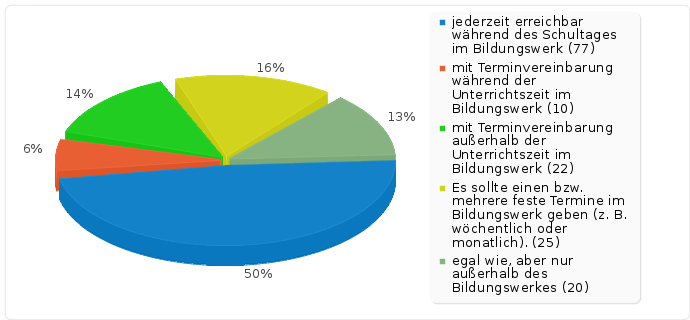
\includegraphics[width=1.0\textwidth]{images/Rahmenbedingungen-fuer-Unterstuetzungangebote.png}
	\caption{Rahmenbedigungen für Unterstützungsangebote}
	\label{fig:Rahmenbedingungen-fuer-Unterstuetzungangebote}
\end{figure}

\noindent
Wie der Grafik zu entnehmen ist wünschen sich $\approx$ 50\% der Schüler eine ständige Erreichbarkeit von Beratungs- und Unterstützungsangeboten am DRK Bildungswerk; $\approx$ 37\% der Befragten plädieren für feste Terminvergaben am Bildungsinstitut und ca. 13\% könnten sich Beratungs- und Unterstützungsangebote nur außerhalb des schulischen Geschehens vorstellen.\\

\noindent
\textbf{Abschnitt 3: Allgemeine Problemlagen im DRK Bildungswerk SN und Annahme außerunterrichtlicher Unterstützungsangebote}\\

\noindent
Nachdem im vorherigen Punkt die persönlichen Probleme und Bedarfe der Schüler im Fokus der Befragung standen, ist nun die Sicht der Schüler auf ihre Mitschüler im Blickpunkt des Interesses.

144 von 154 Schülern, das entspricht $\approx$ 93,5\% aller Befragten, sahen Bedarf für außerunterrichtliche Beratungs- und Unterstützungsangebote am DRK Bildungswerk SN. 10 Schüler sehen kein Bedarf für Angebote und beantworten daher die letzten 4 Fragen dementsprechend.

Die folgenden Problemlagen werden von den Schülern wahrgenommen (Abb.: \ref{fig:Problemlagen-der-Mitschueler}). Diese weisen auf die subjektive Notwendigkeit von außerunterrichtlichen Beratungs- und Unterstützungsangeboten am DRK Bildungswerk SN.

\begin{figure}[ht]
	\centering
		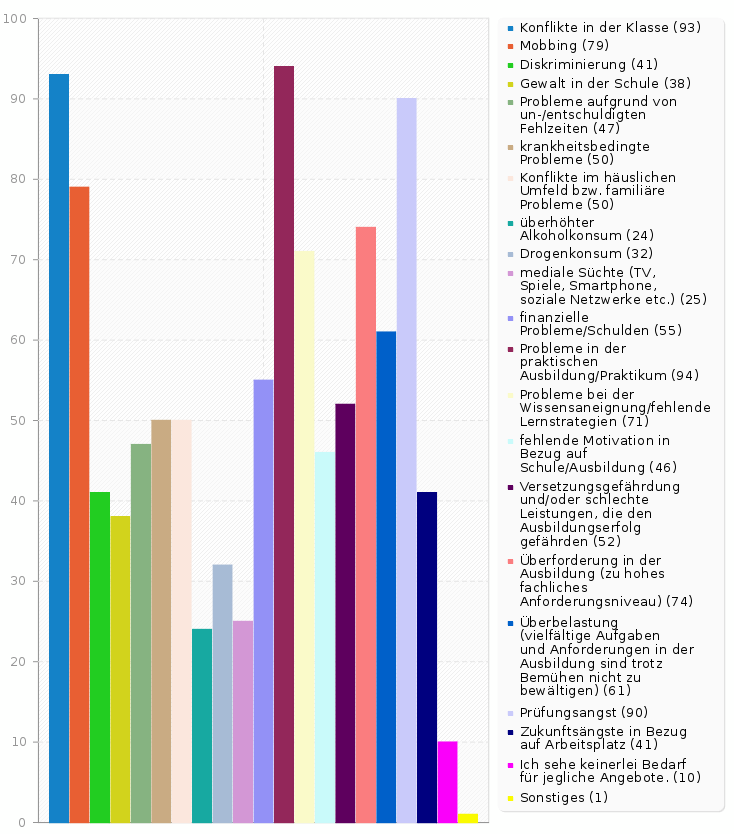
\includegraphics[width=1.0\textwidth]{images/Problemlagen-der-Mitschueler.png}
	\caption{wahrgenommene Problemlagen der Mitschüler, für die außerunterrichtliche Beratungs- und Unterstützungsangebote vorhanden sein sollten}
	\label{fig:Problemlagen-der-Mitschueler}
\end{figure}

\noindent
Im Gegensatz zur persönlichen Sichtweise kommt es hier zu einem signifikanten Anstieg der benannten Problemlagen. Alleinig der überhöhte Alkoholkonsum (24) und die medialen Süchte (25) sind Problemlagen die weniger als 30x (!) angekreuzt wurden. Alle weiteren 17 Probleme wurden massiv angekreuzt. Konflikte in der Klasse (93), Probleme in der praktischen Ausbildung (94) und Prüfungsangst (90) sind hier nur die 3 "`Spitzenantworten"'.

Die Angaben bezgl. Personenkreis und Rahmenbedingungen der außerunterrichtliche Beratungs- und Unterstützungsangebote ähneln der persönlichen Sichtweise und äußern sich wie folgt (Abb.: \ref{fig:Personenkreis-fuer-unterstuetzungsangebote}; Abb.: \ref{fig:Erreichbarkeit-von-Beratungs-und-Unterstuetzungangeboten(2)}). 

\begin{figure}[ht]
	\centering
		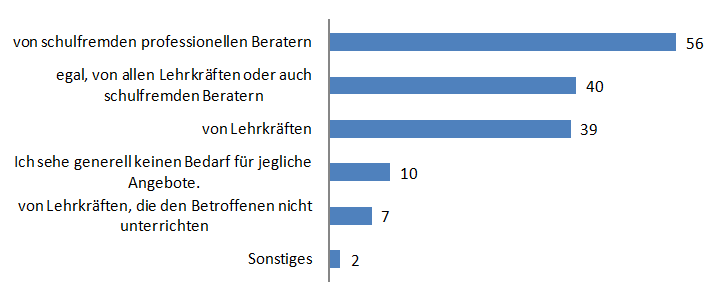
\includegraphics[width=1.0\textwidth]{images/Personenkreis-fuer-unterstuetzungsangebote.png}
	\caption{Personenkreis, welcher Beratungs- und Unterstützungsangebote zur Verfügung stellen sollte}
	\label{fig:Personenkreis-fuer-unterstuetzungsangebote}
\end{figure}

\noindent
Neben der expliziten Nennung der Lehrkräfte (46) sowie schulfremder Berater (56) werden auch beide Parteien als unterstützender Ansprechpartner akzeptiert (40). Eine Differenzierung in Lehrkräfte die die Person unterrichten oder nicht, wird kaum vorgenommen, sowohl in der persönlichen als auch in der allgemeinen Angabe (5 bzw. 7 Nennungen). Daher wurden die unterrichtenden als auch die nicht unterrichtenden Lehrkräfte zahlenmässig im Ergebnis zusammengefasst.

\begin{figure}[ht]
	\centering
		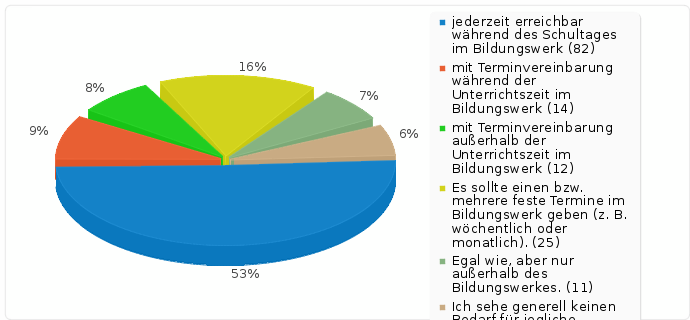
\includegraphics[width=1.0\textwidth]{images/Erreichbarkeit-von-Beratungs-und-Unterstuetzungangeboten(2).png}
	\caption{Erreichbarkeit von Beratungs- und Unterstützungsangeboten}
	\label{fig:Erreichbarkeit-von-Beratungs-und-Unterstuetzungangeboten(2)}
\end{figure}

\noindent
Die Erreichbarkeit der Angebote wird sowohl in der persönlichen als auch in der allgemeinen Angabe annähernd gleich benannt. $\approx$ 53\% befürworten eine ständige Erreichbarkeit am DRK Bildungswerk SN, ca. 33\% fordern feste Terminvergaben und nur 11 Personen ($\approx$ 7\%) erwarten Beratungs- und Unterstützungsangebote außerhalb der schulischen Einrichtung. Die verbleibenden 10 Personen sehen für den gesamten Abschnitt keinerlei Bedarfe.

\newpage
\subsection{Ergebnisdarstellung der Lehrerinterviews}
\label{sec:ErgebnisdarstellungDerLehrerinterviews}

\textbf{Hinweis} 
\begin{itemize}
	\item Grundlage der folgenden Ausführungen ist die Ergebnisdarstellung der universitären Gruppenarbeit \footcite[vgl.]{Hemmerling2015}. Diese wurde überarbeitet und inhaltlich ergänzt (I.04 - I.05).
	 \item Zur besseren Lesbarkeit wurde innerhalb der Ankerzitate auf Pausenangaben und Füllworte verzichtet. Die vollständigen Originalaussagen können jedoch den Transkripten entnommen werden.
	\item Die Unterkategorien wurden mit einem oder mehreren Ankerzitaten belegt, je nach subjektiver Notwendigkeit.
\end{itemize}

\subsubsection{Hauptkategorie A Ausbildungsbeeinflussende Problemlagen}
\label{sec:HauptkategorieAAusbildungsbeeinflussendeProblemlagen}

Die Hauptkategorie "`Ausbildungsbeeinflussende Problemlagen"' fasst in den Unterkategorien alle Problemlagen zusammen, die die Lehrkräfte am DRK Bildungswerk SN subjektiv als ausbildungsbeeinflussend wahrnehmen und die sie in den Interviews benannt haben.\\

\noindent
\textbf{Unterkategorie A.1 Mobbing}\\
\underline{Definition:} Mobbing unter den Schülern wurde von allen befragten Lehrkräften als schwerwiegendes Problem bemerkt und benannt. Es beeinflusst stark das Klassenklima und damit verbunden die Lernatmosphäre. Unter dem Begriff Mobbing wird in diesem Fall jegliche Art des Mobbings verstanden, d. h. sowohl offenes, als auch verstecktes Mobbing gegen einen oder mehrere Schülern sowie das Cybermobbing in sozialen Netzwerken.\\
\underline{Ankerzitat:} "`Im Januar hatten wir einen schlimmen Mobbingfall in der Klasse, mit Beschimpfungen, mit Facebook und Bilder gepostet und so weiter."' (I.03; Z 177--178)\\
\underline{Kodierregel:} Es werden Aussagen kodiert, wenn in ihnen eine der verschiedenen Arten von Mobbing ausgedrückt werden.\\

\noindent
\textbf{Unterkategorie A.2 Fehlzeiten}\\
\underline{Definition:} Fehlzeiten beinhaltet, jedwede \textit{A.2.1 Verspätungen} sowie \textit{A.2.2 entschuldigtes bzw. unentschuldigtes Fehlen} der Schüler in Bezug auf den schulischen Unterricht. Die Gründe, warum Schüler sich verspäten oder erst gar nicht zum Unterricht erscheinen, sind vielfältig und stellen wiederum eigene Problemlagen dar, die in den folgenden Unterkategorien mit aufgegriffen werden. Dazu zählen bspw. Probleme bei der Kinderbetreuung, psychische Probleme, mangelnde Alltagsstrukturen und Desinteresse an der Ausbildung. Fehlzeiten, egal welcher Art, sind problematisch, weil die meisten Prüfungszulassungen eine Mindestanwesenheit zur Teilnahme an der Abschlussprüfung vorschreiben. Die fehlenden Schüler verpassen durch die Fehlzeiten nicht nur relevante Bildungsinhalte in der Schule, sondern riskieren auch eine Nichtzulassung zur Prüfung.\\
\underline{Ankerzitat:} "`wenn Schüler gar nicht kommen. Und sich och ni abmelden, wenn die einfach unentschuldigt fehlen. Und wenn ich dann nachfrage warum. Wenn sie mir dann sagen "`Ach der Unterricht wär' sowieso ni interessant gewesen, na da bin ich ma zu Hause geblieben. Da konnt' ich viel besser lernen"' Das sind meine Lieblingssätze. Denn da kannste die nur erinnern. An ihr'n Ausbildungsvertrag. Dass die regelmäßig und mit Erfolg den Unterricht besuchen müssen."' (I.01; Z 250--254)\\
\underline{Kodierregel:} Es werden Aussagen kodiert, die Verspätungen, Nichterscheinen, entschuldigtes und unentschuldigtes Fehlen sowie Abwesenheit von Schülern beschreiben.\\

\noindent
\textbf{Unterkategorie A.3 Schwangerschaft}\\
\underline{Definition:} Bestehende oder ungewollte Schwangerschaften während der Ausbildung beeinflussen die Fortführung der Ausbildungszeit. Entweder wird die Ausbildung ausgesetzt und zu einem späteren Zeitpunkt wieder aufgenommen oder Schüler brechen sie ganz ab.\\
\underline{Ankerzitat:} "`Oder wenn die schwanger sind, dann sind die och meistens als erstes bei mir. Also von Schwangerschaften in der Physiotherapie erfahr ich als Erste. Naja dann hörste dir das an. Zeigst die Möglichkeiten auf. Entscheiden müssen sie's alleine. Und es gibt ja die Möglichkeit die Ausbildung zu unterbrechen. Das ist ja ni der Akt."' (I.01; Z 391--396)\\
\underline{Kodierregel:} Alle Textstellen, die etwas über Schwangerschaften während der Ausbildung aussagen, werden kodiert.\\

\noindent
\textbf{Unterkategorie A.4 Drogenkonsum und seine Auswirkungen}\\
\underline{Definition:} Es ist bekannt, dass einzelne Schüler verschiedene Arten von Drogen konsumieren und dadurch psychische Probleme haben. Bei anderen Schülern hegen die Lehrpersonen nur den Verdacht des Drogenkonsums, denn sie zeigen auffälliges Verhalten und sind oft kompliziert im Umgang. Der Drogenkonsum wird teilweise auch als eine Form des Ausprobierens im Jugendalter gesehen.\\
\underline{Ankerzitat:} "`sondern einfach dieser Haufen junger Menschen, die sich och ma ausprobiern wolln. Ich denke, da kommt einiges zusammen. Ich hab och bei mir zwei Schüler, is ni meine Klasse, aber zwei Schüler im Verdacht, das die das nehm'. Bei dem ein weiß ich's, dass er Gras raucht, das hat der mir och no erzählt. Wo wir dann gesagt ham "`Mach ma halb lang"'. Und bei dem andern da wees'schs ni. Aber wenn ich dem in de Augen gucke, dann weiß ich schon Bescheid, weil so große Pupillen kann man ni immer ham. Aber du kannst es ja niemandem unterstelln."' (I.01; Z 131--137)\\
\underline{Kodierregel:} Es werden alle Aussagen kodiert, wenn in ihnen Drogen, Drogenkonsum und Auswirkungen des Drogenkonsums thematisiert werden.\\

\noindent
\textbf{Unterkategorie A.5 Ziel- und Orientierungslosigkeit}\\
\underline{Definition:} Die Schüler werden als ziel- und orientierungslos in dem Sinne beschrieben, dass sie nicht wissen, wo ihre Stärken und Schwächen liegen. Damit verbunden fehlen ihnen Ziele, speziell Lebensziele, welche sie erreichen wollen und für die sie sich engagieren würden. Viele Schüler brechen zudem die Ausbildung ab, sobald Probleme auftreten, ein Umstand der ggf. durch mangelnde erzieherische Grenzen im Elternhaus zu erklären wäre. So haben bereits viele Schüler eine oder mehrere Ausbildungen begonnen und abgebrochen und befinden sich in der momentanen Ausbildung nur, weil andere ihnen dazu geraten haben. Insbesondere die pflegerischen Berufe gelten als zukunftssicher, die Potentiale der Schüler liegen jedoch oftmals in ganz anderen Bereichen. Dieser Umstand wird von den Schülern selbst jedoch oft nicht wahrgenommen. Es spiegelt sich nur in dem hohen Ausbildungsabbruch wider.\\
\underline{Ankerzitat:} "`dass is diese Orientierungslosigkeit die manche haben. Das is die Zeit hier absitzen und guckn, wie se, wie se. Die jetz och ni richtig wissen, was se machen könn und was se machen wolln. Und die ham, also ich hab Schüler, die würd ich überall anders sehn, aber ni in der Physiotherapie, weil die ham andre Potentiale, die könntn ganz andre Dinge tun. Aber das is ja häufig so, dass du, wenn du in ner Sache drin steckst und alle redn auf dich ein, dann blockst du ja ab. Die müssen selber dahinter komm, dass es ni rische für se is."' (I.01; Z 162--167)\\
\underline{Kodierregel:} Alle Aussagen, die zu den Themen Ziele und Orientierung für das weitere Leben, Bewusstsein Stärken und Schwächen sowie Gründe für Ausbildungswahl getroffen wurden, werden kodiert. \\

\noindent
\textbf{Unterkategorie A.6 Desinteresse und Demotivation für Ausbildung}\\
\underline{Definition:} Das Desinteresse und die Demotivation für die Ausbildung zeigt sich bei der Vorbereitung der Schüler auf den Unterricht, denn oft haben die Schüler ihre Unterrichtsmaterialien, Lehrbücher, Hausaufgaben etc., nicht dabei. Das Lernen und Behalten von berufsspezifischem Wissen ist bei den Schülern nicht zufriedenstellend und wird ohne große Motivation betrieben. Die Unterrichtszeit wird nicht zum aktiven Lernen genutzt, oft sitzen die Schüler diese Zeit nur ab ohne sich aktiv am Unterrichtsgeschehen zu beteiligen. Ein Grund dafür ist, dass Schüler von Dritten zu dieser Berufsausbildung überredet worden sind und sich selbst gar nicht für diesen Bereich interessieren. Einen anderen Grund bilden die Erfahrungen, die die Schüler in den Praktika gesammelt haben. Die Praxis, in der die Schüler ohne Anleitung nur nebenher laufen müssen, fördert eher die Demotivation und Frustration, welche sich dann in der Schule weiter fortsetzt.\\
\underline{Ankerzitat:} "`Aber man macht’s den Schülern och ni leicht sich zu motiviern. Und wenn die dann im Praktikum immer no hörn müssen "`Lehrjahre sin keine Herrenjahr"'. Orrr, diesen Spruch, hass ich ja wie die Pest. Das wissen die Schüler, das wissen die. Aber das heeßt doch ni, dass se deswegen ständig putzen müssen und einkaufen gehen müssen, die solln fachlich was lern'. Und dann komm se frustriert ausm Praktikum zurück, dann ham se erst gar keine Lust mehr. Das is en rischer Teufelskreis manchma."' (I.01; Z 178--187)\\
\underline{Kodierregel:} Alle Aussagen, die zu den Themen Desinteresse, Demotivation, Frustration durch Praktikum und Nichtteilnahme am Unterricht getroffen wurden, werden kodiert.\\

\noindent
\textbf{Unterkategorie A.7 Schulische Probleme}\\
\underline{Definition:} Das Spektrum der schulischen Probleme ist sehr umfassend, so dass eine weitere Untergliederung in die einzelnen schulischen Probleme sinnvoll war.\\
\textit{A.7.1} Der Unterpunkt \textit{Bezüglich des Fachwissens} umschreibt mehrere Facetten von schulischen Problemen, denen sich Schüler gegenüber sehen. Mangelnde anatomische Grundkenntnisse wirken sich z.B. negativ auf die praktische Anwendung aus und können somit Prüfungsangst erzeugen. Gleichzeitig verlieren die Schüler oft das Interesse am Unterricht, da sie die neuen Bildungsinhalte nicht mit dem vorhandenen Wissen verknüpfen können. Eine weitere Problematik ist die hohe Heterogenität in den Klassen, welche zu Über-- und Unterforderung der einzelnen Schüler führen kann. Zudem beklagen die Lehrkräfte mangelnde Kompetenzen, welche bereits in der allgemeinbildenden Schule hätten vermittelt werden sollen.\\
\textit{A.7.2 Probleme mit Lehrkräften} entstehen aus den verschiedensten Gründen und beeinflussen die Lernatmosphäre negativ.\\
\textit{A.7.3} Einige Schüler sehen sich in der \textit{Prüfungsvorbereitung} in Bezug auf Einordnung der Lernfelder bzw. Schwerpunktsetzung der relevanten Inhalte überfordert.\\
\textit{A.7.4 Unterrichtsbedingungen} sind nicht immer optimal gegeben. Besonders betroffen davon, sind die Schüler die eine berufsbegleitende Ausbildung absolvieren. Neben der normalen 40 Stunden Arbeitswoche wird noch der Unterricht besucht. Es entstehen Konflikte bei der Vereinbarkeit von Berufsleben und Ausbildungszeit sowie zwischen Anspruch und Realität an die Leistungen in der Schule. \\
\textit{A.7.5 Fehlende Lernstrategien} bedeutet, dass die Schüler nicht wissen, wie sie lernen müssen um Wissen optimal zu speichern. Dadurch ist das Wissen nicht abrufbar und sie können es nicht anwenden.\\
\textit{A.7.6 Vermehrtes Auftreten von Lese-Rechtschreib-Schwäche} bedeutet für Schüler und Lehrer ein größerer Zeit- und Materialaufwand, um allen Schülern gerecht werden zu können.\\
\textit{A.7.7 Unterschiedliche Ausprägung der Problemlagen in einzelnen Ausbildungsgängen}
In den verschiedenen Ausbildungsrichtungen im Fachbereich Gesundheit und Pflege treten Probleme der Schüler unterschiedlich stark auf. Welche Problemlagen auftreten ist abhängig vom Ausbildungsgang. Das suggeriert, dass das Auftreten von Problemlagen klientelabhängig ist, d.h. bei Physiotherapeuten gibt es weniger Schüler mit gravierenden Problemen als bspw. bei den Krankenpflegehelfern. Welche Problemlagen auftreten und wie stark sie ausgeprägt sind, könnte indirekt auch mit dem Grad des Bildungsabschlusses zusammenhängen.\\
\underline{Ankerzitate:} (1) "'Viele haben ja auch Angst, gerade in der Manuellen, da kommen die eben vier Minuten später, weil die wissen der Lehrer macht in den ersten vier Minuten Überprüfungen und dann denken die, wenn die nicht da sind, dann kann man mich ja nicht überprüfen und das machen die auch, weil die Angst haben, weil sie es nicht können und warum können sie es nicht? Weil sie die Anatomie nicht kennen und das ist so ein Grundproblem, dass Schüler eben sich auch einige Dinge klemmen, weil sie Angst davor haben. Weil sie Angst davor haben, dran zu kommen, reden zu müssen, und davor haben die eigentlich schon Angst, weil die unsicher sind, nicht weil sie nicht gelernt haben, sondern weil sie einfach noch nicht rausgefunden haben, wie sie lernen müssen."' (I.01; Z 706--715)\\
(2) "'Schüler sind bemüht ihre Leistung, die sie erbringen müssen gut zu machen. Es gelingt dem einen mehr und dem anderen weniger. Ist Tagesformat abhängig. Schwierig ist es, weil die Schüler direkt von der Arbeit kommen. Manche sind 40 Stunden tätig auf Arbeit und kommen danach in die Schule. Und zwar beginnt der Unterricht um 15.30 Uhr und endet um 21.30 für die Schüler. Und das ist im letzten Block von 18.15 Uhr bis 21.30 Uhr sehr beschwerlich für die Schüler."' (I.02; Z 101--106)\\ (3) "'und das spürt man halt och. Das is das heterogene. Wir haben dort Medizinstudentenabbrecher dabei, die schon ne ganz andere Strukturstufe kennengelernt haben und eben welche die sind ganz frisch von der 10. Klasse runtergekommen und gehen jetzt die ersten Schritte selbstständig."' (I.04; Z 61--64)\\
\underline{Kodierregel:} Es werden alle Aussagen kodiert, wenn in ihnen schulische Probleme aller Art ausgedrückt und näher beschrieben werden.\\

\noindent
\textbf{Unterkategorie A.8 Schwieriges familiäres Umfeld}\\
\underline{Definition:} Diese Kategorie wird noch einmal unterteilt in \textit{A.8.1 Grenzerfahrung und Krisenbewältigung} und \textit{A.8.2 Erziehung/sozialer Hintergrund.} Unter Grenzerfahrung und Krisenbewältigung werden alle familiären Krisen z.B. in Form von Krankheiten der Eltern, Suizide, Krankenhausaufenthalte, sowie Maßnahmen von staatlicher Seite in Form des Eingreifens durch das Jugendamt, verstanden. Bei dem Punkt Erziehung/sozialer Hintergrund spielen Faktoren wie Erziehungsstil, Vermittlung von Werten und Normen sowie aktuelle Wohn- und Lebensverhältnisse der Schüler eine wichtige Rolle. Beide Bereiche können eine Vorhersage geben, inwieweit der Schüler in der Lage ist, eine Ausbildung erfolgreich zu beenden.\\
\underline{Ankerzitat:} "`Problemlage ist auf jeden Fall das Elternhaus. Das also dieses Modelllernen von Normen und Werten, dass findet teilweise gar nicht statt, zumindest nehm ich das so wahr, no?, dass es auch gar nicht vermittelt wurde pünktlich zu sein, höflich zu sein und so weiter. Das natürlich auch in der Vergangenheit bei den Schülern ganz viele Krisen bestanden, sei's vom Suizid des Bruders bis hin zu Krankenhausaufenthalten, Schlaganfall der Mutter. Also wir hatten schon wirklich Vieles, bis hin zur Einschreitung des Jugendamtes."' (I.03; Z 115--120)\\
\underline{Kodierregel:} Alle Textstellen, die etwas über Erziehung, Verhältnis Schüler-Eltern, sozialen Hintergrund, Krisen und Grenzerfahrungen innerhalb der Familie ausdrücken, werden kodiert.\\

\noindent
\textbf{Unterkategorie A.9 Probleme im und mit Praktikumseinsatz}\\
\underline{Definition:} Aufgrund potentieller Schwierigkeiten im Praktikumseinsatz, bspw. bedingt durch das Hierarchiegefälle im Krankenhaus, negativer Beurteilung oder undifferenzierter Aufgabenzuteilung, reagieren die Schüler mit Abwesenheit, persönlicher Distanz und Praktikumswechsel. Der sofortige Arbeitgeberwechsel kann dabei als Form des individuellen Umgangs mit Kritik oder Problemen angesehen werden. Das löst die Probleme aber nicht, sondern verursacht weitere, siehe \textit{A.6 Desinteresse und Demotivation}. Zudem versuchen Schüler die Schule und den Praxisbetrieb gegeneinander auszuspielen um sich persönliche Vorteile zu verschaffen.\\
\underline{Ankerzitate:} (1) "'in Praktika, in den Krankenhäusern, wenn da Schwestern oder Ärzte vielleicht ja den KPH's anders entgegen getreten sind. Das Hierarchiegefälle eben sehr hoch war, dann reagieren die Schüler meistens mit Abwesenheit, mit Distanz, mit ja, das sie direkt gleich das Praktikum wechseln wollen"' (I.03; Z 136--140)\\ (2) "'da sind wir wieder bei dem Problem die Vorteile zu festigen um dann zu sagen: "`In der Schule die haben uns das so gesagt und in der Praxis müsst ihr's wieder so machen."' Also diese Rivalität, die dann entsteht. Also och gegeneinander aufreiben und hier die schönen Dinge rauspicken um das dann draußen einzufordern und draußen die schönen Dinge wieder aufzupicken um die hier einzufordern."' (I.04; Z 208--212)\\
\underline{Kodierregel:} Es werden Aussagen kodiert, in denen Probleme im oder mit dem Praktikum beschrieben werden.\\

\noindent
\textbf{Unterkategorie A.10 Probleme bei der Kindererziehung und -betreuung}\\
\underline{Definition:} Probleme bei der Kindererziehung umfasst alle Probleme, die durch schwierige Lebenssituationen, psychiatrische und andere Erkrankungen, Verlusterfahrungen oder Verhaltensauffälligkeiten ausgelöst werden. Probleme bei der Kinderbetreuung bedeutet, dass Unterrichtszeit verpasst wird, weil Kinder selbst betreut werden müssen, da kein Anderer diese Aufgabe übernehmen konnte oder wollte. \\
\underline{Ankerzitat:} "`Haben alle Kinder. Also fast alle Kinder. mit ihren Problemen. Was die Erziehung angeht. persönliche/schwierige Lebenslagen/psychiatrische Erfahrungen oder Grenzerfahrungen mit ihren Kindern sowie wenn sich ein Kind eigenartig verhält, ob es vielleicht wichtig ist jetzt jemanden einzuschalten, einen Professionellen einzuschalten. Oder ob man das im Rahmen der Familie lösen kann."' (I.02; Z 148--153)\\
\underline{Kodierregel:} Alle Textstellen, die etwas über die Kindererziehung, Erkrankungen oder Auffälligkeiten der eigenen Kinder sowie der Kinderbetreuung aussagen, werden kodiert.\\

\noindent
\textbf{Unterkategorie A.11 Probleme in der Partnerschaft}\\
\underline{Definition:} Beziehungsprobleme beeinflussen die Ausbildung dahingehend, dass der schlechte Einfluss oder die Unzuverlässigkeit des Partners zu einer Vernachlässigung der Ausbildung führt. Auch Ausbildungsabbrüche werden aufgrund von partnerschaftlichen Problemen in Erwägung gezogen.\\
\underline{Ankerzitat:} "`der Freund hat sich getrennt. Haha, das ist schlimm. Das ist wirklich schlimm. Da, will man die Ausbildung hinwerfen."' (I.01; Z 383--386)\\
\underline{Kodierregel:} Alle Aussagen, die partnerschaftlichen Probleme jeglicher Art thematisieren, werden kodiert.\\

\noindent
\textbf{Unterkategorie A.12 Finanzielle Probleme}\\
\underline{Definition:} Viele Ausbildungsgänge sind schulische Vollzeitausbildungen, d.h. dass es keinen dualen Partner gibt, welcher den Schülern ein Ausbildungsgehalt zahlt. Deshalb müssen viele Schüler neben dem Schulbesuch arbeiten um ihren Lebensunterhalt finanzieren zu können.\\
\underline{Ankerzitat:} "`wir sind ja eine Zentralausbildung, dass sie sich meistens noch was zum Lebensunterhalt dazu verdienen."' ( I.01; Z 620--621)\\
\underline{Kodierregel:} Alle Textstellen, die etwas über die finanzielle Situation der Schüler aussagen, werden kodiert.\\

\noindent
\textbf{Unterkategorie A.13 Gesundheitliche und krankheitsbedingte Problemlagen}\\
\underline{Definition:} Es wird ein Zusammenhang zwischen dem Auftreten verschiedener Erkrankungen und dem sozialen Status der Schüler vermutet. Schüler mit einem niedrigen sozialen Status haben somit ein höheres Risiko zu erkranken. Das wird belegt, durch das vermehrte Auftreten von Erkrankungen wie Magenbluten, Depression, Schizophrenie oder allgemeinen psychischen Auffälligkeiten, bei Schülern aus einem schwierigen sozialen Umfeld. Diese Schüler wurden häufig bereits in der allgemeinbildenden Schule von Schulpsychologen betreut.\\
\underline{Ankerzitat:} "`ich hab den Eindruck, das ist aber natürlich nicht wissenschaftlich belegt, dass diese Schüler mit diesen niedrigen sozialen Status auch viel höhere Erkrankungsrisiken haben. Also das, das heißt ich, ja dass grad in dem jungen Alter schon ganz viele Erkrankungen schon aufgetreten sind. Sei's von Magenbluten bis hin zu Depression, Schizophrenie, das ist alles nur in der Klasse."' (I.03; Z 122--126)\\
\underline{Kodierregel:} Es werden alle Aussagen kodiert, in welchen spezifische Erkrankungen, Erkrankungsrate sowie Erkrankungsrisiko im Zusammenhang mit dem sozialen Stand der Schüler ausgedrückt werden.\\

\noindent
\textbf{Unterkategorie A.14 Differenz von Selbst- und Fremdwahrnehmung}\\
\underline{Definition:} Unter der Differenz von Selbst- und Fremdwahrnehmung in Schule und im Praktikum wird verstanden, dass Schüler nicht einschätzen können, wo ihre Stärken und Schwächen liegen. Der Umgang mit Problemen, persönlicher Kritik oder schulischen Misserfolg fällt vielen Schüler schwer. Sie reagieren daraufhin mit unreflektierten, erkenntnisresistenten und nicht altersgerechten Verhalten. Das äußert sich bspw. darin, dass Schüler im Unterricht verstärkt auf Aufmerksamkeit und positive Bestätigungserlebnisse drängen. Diverse Probleme werden zudem nicht als Problem wahrgenommen. Desweiteren kommt es aufgrund fehlender Integrationsfähigkeiten einzelner Schüler zu klasseninternen Konflikten. Ungenügende Sozialkompetenz und mangelnde Akzeptanz der Schülerrolle führen zu weiteren Diskrepanzen.\\
\underline{Ankerzitate:} (1) "'der hat ein völlig falsches Bild von sich. Da stimmen Selbstwahrnehmung und Fremdwahrnehmung nirgendwo überein, weder hier in der Schule, noch im Praktikum. Mit dem haben wir immer mal Probleme im Praktikum, dass der distanzlos ist, dass der denkt, er wäre der große Bringer, aber wenn man dann mal hinterfragt, weiß er dann nicht wirklich irgendwas."' (I.01; Z 83--86)\\ (2) "'das sind so ganz klar, das sind och mit die meisten Problemkinder weil die eben och im Unterrichtsgeschehen dann so diese Aufmerksamkeit fordern bzw.  wenn sie die ni kriegen, dann eben och gleich wieder zumachen und dann die Bockigen sin."' (I.04; Z 118--120)\\
\underline{Kodierregel:} Alle Textstellen, die etwas über die Selbst- und Fremdwahrnehmung von Schülern sowie das Agieren in der Rolle als Schüler aussagen, werden kodiert.\\

\noindent
\textbf{Unterkategorie A.15 Verlusterfahrung / Trauer}\\
\underline{Definition:} Die Schüler erfahren Verluste in der Klasse und müssen mit ihrer Trauer umgehen lernen. Der Verlust eines Mitschülers ist für manche Schüler der Erstkontakt mit dem Thema Tod und Sterben.\\
\underline{Ankerzitat:} "`eine Schülerin der Klasse verstorben in diesem Jahr. Ganz plötzlich. Und das warn so einige Höhen und Tiefen in der Klasse, die ja ganz schön reingehaun ham."' (I.02; Z 60--63)\\
\underline{Kodierregel:} Es werden alle Aussagen kodiert, die Verlusterfahrungen und Trauer thematisieren.\\

\noindent
\textbf{Unterkategorie A.16 Ausgeprägte Heterogenität in den Klassen}\\
\underline{Definition:} Ausgeprägte Heterogenität in den Klassen macht sich durch Unterschiede in Herkunft, Religion, Alter, Familienstand sowie persönlichen und beruflichen Voraussetzungen bemerkbar. In einigen Ausbildungsrichtungen wird jeder verfügbare Schüler für eine Ausbildung zugelassen, unabhängig von den Voraussetzungen oder der persönlichen Eignung für den Beruf. Diese Heterogenität führt zu Gruppenbildungen innerhalb der Klasse und beeinflusst die Ausbildung teilweise negativ.\\
\underline{Ankerzitat:} "`ich glaub die Jüngste ist 17 und der Älteste 45; dann sind die Multikulti, alles aus verschiedenen Nationen und verschiedenen Herkünften, von der Religion auch verschieden; manche haben auch schon Familie, manche sind halt frisch von der Schulbank und auf der einen Seite ist das interessant, off auf der anderen Seite ist das manchmal auch schwierig die alle unter'n Hut zu bringen weil halt viele Gruppen in der Klasse sind dadurch."' (I.05; Z 34--39)\\
\underline{Kodierregel:} Es werden alle Aussagen kodiert, welche die Heterogenität in der Klasse thematisieren.

\subsubsection{Hauptkategorie B Einfluss der Problemlagen auf den Unterricht}
\label{sec:HauptkategorieBEinflussDerProblemlagenAufDenUnterricht}

Die Hauptkategorie B beschreibt die Auswirkungen der privaten Problemlagen der Schüler auf den Unterricht. Dabei wird der Begriff "`Unterricht"' hier eher weit gefasst, d.h. neben der klassischen Unterrichtsstunde zählen hier auch Beeinträchtigungen in schulischen Praktika dazu. Der grundlegend eher negative Tenor der Beeinflussung durch Demotivation, fehlende oder mangelnde Mitarbeit, Fehlzeiten oder Beeinflussung durch Mitschüler wird durch den Punkt \textit{"`positive Beeinflussung des Unterrichtsgeschehens"'} abgemildert. Hierbei handelt es sich um Erfahrungen der Schüler in Bezug auf private Problemlagen ihrerseits, welche als Zugewinn für einen Austausch im Unterrichtsgespräch angesehen werden. Des Weiteren werden unter diesem Punkt auch Einflüsse der privaten Problemlagen der Schüler auf den Alltag der Lehrer dargelegt (Unterrichtsplanung, Störung des Unterrichtsablaufs, Störung der Lehrperson).\\

\noindent
\textbf{Unterkategorie B.1 Negative Auswirkungen der Problemlagen auf das Praktikumsgeschehen}\\
\underline{Definition:} In dieser Unterkategorie werden die Auswirkungen der persönlichen Problemlagen auf außerschulische Praktikumseinsätze der Schüler beschrieben. Eine nähere Definition der zugrunde liegenden Problemlagen findet dabei nicht statt.\\
\underline{Ankerzitate:} (1) "'Mit dem haben wir immer mal Probleme im Praktikum, dass der distanzlos ist, dass der denkt, er wäre der große Bringer, aber wenn man dann mal hinterfragt, weiß er dann nicht wirklich irgendwas."' (I.01; Z 84--85)\\ (2) "'Der hat ja jetzt, im letzten Praktikum war das ganz extrem, der hat sogar Patienten vergrault."' (I.01; Z 89--90)\\ (3) "' [\punkte] in Praktika, in den Krankenhäusern, wenn da Schwestern oder Ärzte vielleicht ja den KPH's anders entgegen getreten sind. Das Hierarchiegefälle eben sehr hoch war, dann reagieren die Schüler meistens mit Abwesenheit, mit Distanz, mit ja, das sie direkt gleich das Praktikum wechseln wollen [\punkte] (I.03; Z 136--140)\\
\underline{Kodierregel:} Alle Textstellen, die die Auswirkungen von Problemlagen in Praktikumseinsätzen beschreiben, werden hier aufgeführt.\\

\noindent
\textbf{Unterkategorie B.2 Mangelnde Mitarbeit}\\
\underline{Definition}: Die Problemlagen der Schüler stellen sich mannigfaltig im Unterricht dar. Von den Lehrern häufig beschriebene Auswirkungen betreffen die Mitarbeit im Unterricht, Demotivation hinsichtlich der Ausbildung und der Bildungsinhalte im Unterricht sowie die sinkende bzw. fehlende Konzentration im Unterricht. Diese Unterkategorie teilt sich wie folgt auf:\\
\textit{B.2.1 Durch Desinteresse an Bildungsinhalten und Demotivation:} Die Problemlagen der Schüler wirken sich massiv auf das Unterrichtsgeschehen aus. In diesem Zusammenhang wird Desinteresse an Bildungsinhalten und eine allgemeine Demotivation der Schüler von den Lehrern als unterrichtsbeeinflussend benannt. Ein Grund hierfür könnte das mangelnde Interesse an der beruflichen Tätigkeit darstellen.\\
\underline{Ankerzitat:} "`Aber die finden weder die, die Pflege der Leute gud, noch finden se de Schule gud. Die finden's nur gut, schöne Fingernägel zu ham und mit ihrm Handy zu spieln. Also dieses Desinteresse is für mich ne große Problemlage."' (I.01; Z 120--122)\\
\textit{B.2.2  Sinkende Motivation und Konzentration:} Die Lehrkräfte konstatieren Auswirkungen der persönlichen Problemlagen welche sich in einer Minderung der Konzentrationsfähigkeit der betroffenen Schüler darstellt. Sie erkennen Konzentrationsminderungen im Unterricht und bei der praktischen Arbeit. Die beschriebenen Konzentrationsschwächen wirken sich im weiteren Lernprozess negativ auf die Motivation der Schüler und auf deren Lernerfolg aus.\\
\underline{Ankerzitate:} (1) "'Das beeinflusst die Motivation ganz stark und das beeinflusst auch den, den Lern-erfolg im Enddefekt"' (I.03; Z 151--152)\\ (2) "'(Sie) ham ihre privaten Probleme, logisch lagert sich das immer auf die Ausbildung ab, auf die Konzentration, auch auf die Lernbereitschaft."' (I.02; Z 180--181)\\
\textit{B.2.3 Fehlende Lernstrategien} führen zu Angst und verminderter Mitarbeit Das bereits beschriebene Desinteresse an Bildungsinhalten und persönlicher Ausbildung seitens der Schüler hat die verschiedensten Gründe. Fehlende Lernstrategien und damit die fehlende Möglichkeit weiterführende Inhalte zu erfassen, wird von den Lehrkräften als eine Ursache für diesen Umstand angesehen. Daraus resultierend kommt es Angstgefühlen, insbesondere zu Versagensangst bei mündlichen Prüfungen, welche zu Unterrichtsbeginn stattfinden. Die Schüler kommen daher absichtlich zu spät zum Unterricht um bei Wiederholungsprüfungen nicht anwesend zu sein (siehe B.4.2 und B.6)\\
\underline{Ankerzitat:} "`Viele haben ja auch Angst, gerade in der Manuellen, da kommen die eben vier Minuten später, weil die wissen der Lehrer macht in den ersten vier Minuten Überprüfungen und dann denken die, wenn die nicht da sind, dann kann man mich ja nicht überprüfen und das machen die auch, weil die Angst haben, weil sie es nicht können und warum können sie es nicht? Weil sie die Anatomie nicht kennen und das ist so ein Grundproblem, dass Schüler eben sich auch einige Dinge klemmen, weil sie Angst davor haben. Weil sie Angst davor haben, dran zu kommen, reden zu müssen, und davor haben die eigentlich schon Angst, weil die unsicher sind, nicht weil sie nicht gelernt haben, sondern weil sie einfach noch nicht rausgefunden haben, wie sie lernen müssen."' (I.01; Z 706--715)\\
\underline{Kodierregel:} Hier beschriebene Unterkategorien beinhalten alle Textstellen, die Demotivation, verminderte oder fehlende Mitarbeit oder Konzentrationsschwächen beschreiben, welche Auswirkungen auf den Unterricht haben.\\

\noindent
\textbf{Unterkategorie B.3 Positive Auswirkungen auf den Unterricht}\\
\underline{Definition:} Laut Aussage der Lehrkräfte können Schüler, welche früher oder aktuell mit Problemlagen konfrontiert sind bzw. waren, den Unterricht mit ihren diesbezüglichen Erfahrungen vervollkommnen. Sie beschreiben eine positive Beeinflussung des zu behandelnden Themas durch die Nutzung von thematisch passenden Problemlagen (z.B. Krisenbewältigung, Umgang mit Sterben und Tod, Erbkrankheiten) und eine damit verbundene Bereicherung des Unterrichtsgeschehens. Positiv bewertet wird zudem die Zusammenarbeit von Schülern, welche zum Zwecke der schulischen Gruppenarbeit, persönliche Konflikte ausblenden können.\\
\underline{Ankerzitate:} (1) "'Und das beeinflusst den Unterricht dann aber positiv, dadurch dass halt se halt eigene Erfahrungen mit einbringen könn'."' (I.02; Z 191--192)\\ (2) "'Ja mit dem mit der Verlusterfahrung durch den Tod der Schülerin das war natürlich och was was den Unterricht in dem Sinne ja ergänzt hat, wenns darum geht Krisenbewältigung, Umgang mit Tod und Sterben, das ham wa aufgegriffen."' (I.02; Z 194 -196)\\
\underline{Kodierregel:} Alle persönlichen Problemlagen der Schüler, welche sich positiv auf den Unterricht ausgewirkt haben, finden in diesem Absatz Beachtung.\\

\noindent
\textbf{Unterkategorie B.4 Störung des Unterrichtsgeschehens}\\
\underline{Definition:} Diese Unterkategorie beschreibt Unterrichtsstörungen, die durch persönliche Problemlagen der Schüler entstehen und das Unterrichtsgeschehen negativ beeinflussen. Diese wurden wie folgt untergliedert: \\
\textit{B.4.1 Störung des Unterrichtsablaufs:} Aufgrund von einzelnen Schülergesprächen kommt es zu mangelnder Aufmerksamkeit innerhalb der ganzen Klasse, was durch das zu spät kommen einiger Schüler noch verstärkt wird. Die Lehrkräfte fordern in diesem Zusammenhang konsequentere Maßnahmen um diese Störungen zu reduzieren \\
\textit{B.4.2 Störung der Mitschüler:} Auch Mitschüler fühlen sich durch die Auswirkungen von persönlichen Problemlagen im Unterricht gestört. Laut Befragung kritisieren selbst die Schüler die Unterrichtsstörungen durch das häufige Zuspätkommen einiger Mitschüler.\\
B.4.3 Störung der Lehrperson Lehrpersonen berichten, dass insbesondere das unentschuldigte Fehlen sowie die Benutzung des Mobiltelefons im Unterricht einen hohen persönlichen Störfaktor darstellen. \\
\underline{Ankerzitate:} (1) "`Ja, das fängt an, das mein Unterricht selten ungestört ablaufen kann, das heißt es sind immer wieder Gespräche, in, in der Klasse auch mit Ermahnungen oder es sind Abmahnungen zur schriftlichen Abmahnung geht das dann, aber teilweise ohne Konsequenz."' (I.03; Z 167--169)\\ (2) "`Es beeinflusst dahingehend das Schüler permanent fünf Minuten zu spät kommen. Was weniger mich stört als die Mitschüler. Also das zu spät kommen stört mehr die Anderen."' (I.01; Z 242--243, 249)\\ (3) "`Die ist anders. Die ist streng. Wenn da einer zu spät kommt, gibt’s ne Kopfwäsche. Na weil die das immens stört, wenn jemand zu spät kommt."' (I.01; Z 353--355)\\ (4) "'was mich stört ist, wenn Schüler gar nicht kommen. Und sich och ni abmelden, wenn die einfach unentschuldigt fehlen."' (I.01; Z 249--250)\\ (5) "`Wenn die dann einfach so dasitzen. Und dann holn die ihre Handys raus. Wird da getippt und gemacht und getan. Das stört mich. Das Getippe das stört mich."' (I.01; Z 263--264)\\
\underline{Kodierregel:}  Alle Störungen auf das Unterrichtsgeschehen oder daran teilhabende Personen durch persönliche Problemlagen von Schülern wurden berücksichtigt.\\

\noindent
\textbf{Unterkategorie B.5 Verlust von Unterrichtszeit durch Problemlagen der Schüler}\\
\underline{Definition:} Die interviewten Lehrpersonen berichten, dass durch das Übernehmen von beratenden, klärenden, intervenierenden oder schlichtenden Tätigkeiten im Unterrichtsverlauf eine gewisse Zeit einzuplanen ist, welche nicht für Bildungsinhalte oder Kompetenzentwicklung im Rahmen des Lehrplans genutzt werden kann. So wird bspw. durch Trauerarbeit, unpassende Zwischenfragen, Unstimmigkeiten bei der Gruppenbildung oder spezielle persönliche Befindlichkeiten von Schülern der Unterrichtsbeginn oder -ablauf verzögert. Sobald die Lehrkraft auf spezielle persönliche Problemlagen wie Lese-Rechtschreib-Schwächen von Schülern eingeht, muss der verbleibende Unterrichtsstoff dafür umso intensiver und zeitlich gerafft vermittelt werden. Eine weitere Herausforderung für die Lehrkraft sind Schüler, welche mehr mit der eigenen Person als der aktiven Unterrichtsteilhabe beschäftigt sind.\\
\underline{Ankerzitate:} (1) "`Auch im Rahmen des Unterrichts, wo dann teilweise Unterricht ausfallen musste, weil wir als Klasse gemeinsam Trauerarbeit geleistet haben."' (I.02; Z 70--71)\\ (2) "`Da ist man als Lehrer, wenn es darum geht, den Unterricht schnell durchzubringen und viele Lehrinhalte zu vermitteln manchen Tages auch ausgebremst, weil man sich auf die Befindlichkeiten der Schüler einstellt."' (I.02; Z 110--112)\\
\underline{Kodierregel:} Alle die Unterrichtszeit negativ beeinflussenden Problemlagen der Schüler wurden in dieser Unterkategorie berücksichtigt.\\

\noindent
\textbf{Unterkategorie B.6 Fernbleiben vom Unterricht}\\
\underline{Definition:} Hier werden komplette Fehltage thematisiert, welche aufgrund von persönlichen Problemlagen der Schüler entstehen. Diese wirken sich negativ auf die Planung und Umsetzung der Unterrichtseinheiten aus. Des Weiteren haben sie Einfluss auf den Erfolg der Ausbildung der Schüler aufgrund der vorgeschriebenen Höchst-Fehltagezeiten.\\
\underline{Ankerzitate:} (1) "'Wir haben eine hohe Abwesenheitsrate. Also ich hab mal so gerechnet es sind knapp 30\% Abwesenheit pro Tag. Hat den Grund, dass die Schüler in der Theorie keine quasi nicht da sein müssen. Also es gibt keine Zahl, die in der Theorie festlegt, so und so viele Tage dürfen die fehlen um zur Prüfung zugelassen zu sein. Die Tage beziehen sich nur auf die Praxis. Da sind's 35 Praxisfehltage. Wer auch immer das entschieden hat. Ja und das hat den Grund, dass viele Schüler abwesend sind, unentschuldigt fehlen. Ja auch dieses Verfahren mit Krankschreibung, wann muss welche Krankschreibung wohin, dass ist bis heute noch nicht so richtig gefruchtet."' (I.03; Z 79--86)\\ (2) "'Und von diesen bestehenden 17 Schüler sind durchschnittlich 11/12 pro Tag da."' (I.03; Z 109)\\
\underline{Kodierregel:} Es werden alle Textstellen berücksichtigt, welche das Fernbleiben vom Unterricht thematisieren.\\

\noindent
\textbf{Unterkategorie B.7 Einfluss auf Unterrichtsplanung}\\
\underline{Definition:} Persönliche Problemlagen der Schüler beeinflussen das schulische Geschehen auf vielfältige Art. Lehrkräfte müssen die Problemlagen ihrer Schüler daher bei der Planung des Unterrichts stets berücksichtigen, auch wenn das aufgrund der Heterogenität in den Klassen eine große Herausforderung darstellt und nicht immer umgesetzt werden kann. Beispiele der Anpassung an die Bedarfe der Schüler offenbaren sich z.T. in der Umstrukturierung des Unterrichts, im erhöhten Zeitaufwand für die Wissensvermittlung oder in der verstärkten Wiederholung. Eine Lehrkraft legt bspw. theoretische Phasen in die Morgenstunden, den Praxisteil in den Nachmittag und umgeht somit nach eigenen Angaben die Demotivation und sinkende Konzentrationsfähigkeit der Schüler.\\
\underline{Ankerzitate:} (1) "'Es beeinflusst natürlich meinen Unterricht auch so, dass ich die Inhalte ganz anders anlege, das heißt, wenn ich weiß, dass ich acht Stunden Unterricht bei der Klasse am Tag hab, weiß ich, das ab um 12 keine, kein Frontalunterricht mehr möglich ist. Keine Wissensvermittlung, sondern Festigung, Wiederholungen, praktische Inhalte da eher angesagt sind."' (I.03; Z 183--188)\\ (2) "'Schüler brauchen mehr Zeit, auf jeden Fall, auch für die Wissensvermittlung, brauchen mehr Zeit zum Aufschreiben, weil wir auch viele mit Lese-Rechtschreib-Schwächen da, da drin haben. Ja die brauchen immer wieder Wiederholungen, jede Stunde brauchen die ne Wiederholung von Themenbereichs, sonst in den Leistungskontrollen sowohl praktisch als auch theoretisch sieht man dann, dass wenig hängengeblieben ist."' (I.03; Z 188--193)\\ (3) "'Da is man als Lehrer ja, wenn es darum geht, den Unterricht schnell durchzubringen und viele Lehrinhalte zu vermitteln manchen Tages auch ausgebremst, weil man sich wirklich auch auf die Befindlichkeiten der Schüler einstellt."' (I.02; Z 110--112)\\
\underline{Kodierregel:} Es werden alle Aussagen kodiert, die sich auf den Einfluss der persönlichen Problemlagen der SuS auf die Unterrichtsplanung beziehen.\\

\noindent
\textbf{Unterkategorie B.8 Unterrichtsbeeinflussung durch klasseninterne Konflikte}\\
\underline{Definition:} Die persönlichen Problemlagen der Schüler führen zu klasseninternen Konflikten welche den Unterricht negativ beeinflussen. Die Kenntnisnahme der Probleme einzelner Schüler durch die Mitschüler kann zur Ausgrenzung der betroffenen Person, einem unfreundlichen Umgang oder einer allgemein angespannten Stimmung im Klassenverband führen.\\
\underline{Ankerzitat:} "`Dadurch das die alle Ihre Probleme sehr öffentlich in der Klasse auch aus-leben, also das wurde dann auch öffentlich besprochen, egal ob bei Facebook oder die anderen Sachen werden halt schnell auch welche ausgegrenzt, ne. Und viele hinterfragen ja auch ni die Hintergründe, warum, jemand so was macht und somit haben wir och schnell auch Außenseiter."' (I.05; Z 112--115)\\
\underline{Kodierregel:} Es werden alle Aussagen berücksichtigt, welche eine Unterrichtsbeeinflussung durch klasseninterne Probleme thematisieren.

\subsubsection{Hauptkategorie C Erwartungen der Schüler an die Lehrkräfte}
\label{sec:HauptkategorieCErwartungenDerSchülerAnDieLehrkräfte}

Diese Kategorie beschreibt die Erwartungen der Schüler, wenn diese aufgrund ihrer Problemlagen an die Lehrkräfte herantreten. Die interviewten Lehrkräfte sind sich einig, dass die Schüler keine übersteigerte Erwartungshaltung haben und daher keine Problemlösung von Ihnen erwartet wird. Die Schüler sind vielmehr Ratsuchende, welche sich eine zweite Meinung zu einem Thema einholen möchten oder einen Menschen aufsuchen dem sie vertrauen. Für viele Schüler ist der Lehrer zudem die einzige Person, der Ihnen zuhört und sich die Zeit nimmt mit ihnen über ihre Probleme zu reden.\\

\noindent
\textbf{Unterkategorie C.1 Keine Problemlösung}\\
\underline{Definition:} Viele Schüler haben wenige bis gar keine Erwartungen in Bezug auf die Lösung ihrer Problemlagen wenn sie an die Lehrkraft herantreten. Davon abgesehen haben die interviewten Lehrpersonen verschiedene individuelle Formen des Umgangs wenn Schüler mit privaten Problemen auf sie zukommen. Der erste verweist Schüler mit privaten Problemen an andere Ansprechpartner weiter, der Zweite bietet lieber keine Lösung an, um anschließend nicht auf diese Aussage festgenagelt zu werden, ein Dritter nimmt sich Zeit und hört zu und der Andere geht vielleicht wieder anders mit den Problemlagen um.\\
\underline{Ankerzitate:} (1) "'Ich glaube die erwarten nich die Lösung ihrer Probleme. So kommt's mir jedenfalls ni vor."' (I.01; Z 448--449)\\ (2) "'Ja, ob da eine Erwartung dahinter steckt, ob die Probleme gelöst werden können zusammen, das, das weiß ich nicht. Was so private Probleme angeht da will ich mich da nicht dazu äußern, was ich empfehlen würde, weil das, glaube ich zu weit gehen würde, no? Sonst wär glaube ich die Nähe zwischen Schüler und Lehrer zu, zu eng. Kann das zwar thematisieren, aber Lösungsstrategien oder sich in dieses private Leben mit zu involvieren, das wäre mir zu weit."' (I.03; Z 204--212)\\ (3) "'Ich hüte mich auch davor, Lösungen anzubieten. Also ich zeige höchstens ma en Weg, oder die verschiedenen Möglichkeiten auf, weil ich möchte ni am Ende dann da stehn als derjenige, der gesagt hat, dass [\punkte]."' (I.01; Z 450--453)\\
\underline{Kodierregel:} Alle Aussagen. in welchen die Schüler keine Lösung ihrer Problemlagen erwarten oder die Interviewten keine klare Erwartungshaltung hinsichtlich der Schüler formulierten, werden berücksichtigt.\\

\noindent
\textbf{Unterkategorie C.2 Meinung und Rat einholen}\\
\underline{Definition:} Die Lehrkräfte berichten, dass die Schüler sich bei ihnen bezüglich ihrer Problemlagen einen speziellen Rat bzw. eine zweite Meinung einholen möchten. Sie betonen dabei die geforderte Objektivität dieses Rats bzw. Meinung.\\
\underline{Ankerzitate:} (1) "'Die erwarten höchstens von mir, dass ich mal für sie da bin, wie gesagt, dass wir mal unter vier Augen reden können."' (I.01; Z 484--485)\\ (2) "'da bitten sie mich dann [\punkte] da einfach auch nochma ne ne außenstehende Meinung zu bekomm. Das ich da nochma Stellung nehme."' (I.02; Z 157--158)\\ (3) "`[\punkte] und erwarten dann auch ne ganz objektive Meinung und auch nen Rat, in die Richtung."' (I.02; Z 213)\\
\underline{Kodierregel:} Alle Textstellen die das Thema "`Rat geben"' und "`Meinung einholen"' als Erwartungshaltung der Schüler an die Lehrer thematisierte, wurden kodiert. \\

\noindent
\textbf{Unterkategorie C.3 Schüler suchen Personen zum Zuhören}\\
\underline{Definition:} Die Interviewten berichten, dass Schüler mit Problemlagen an sie herantreten, um sich ihre Probleme primär "`von der Seele zu reden"', ein Aspekt der privat oft nicht erfüllt wird. Sie wenden sich an eine vertrauensvolle Person, die Ihnen Aufmerksamkeit schenkt und in einem ungestörten Rahmen persönliche Hinweise und Ratschläge erteilt. Der Klassenlehrer ist meist der erste Anlaufpunkt für betroffene Schüler. Von den aufgesuchten Lehrkräften wird erwartet, dass sie sich Zeit für die Belange der Schüler nehmen und einfach zuhören.\\
\underline{Ankerzitate:} (1) "`Die brauchen nur jemanden der ihnen zu hört, weil sie mit bestimmten Dingen nicht mehr zu ihren Eltern gehen oder mit Freunden im privaten Freundeskreis sprechen."' (I.01; Z 461)\\ (2) "`Ich glaub die erste Erwartung ist erst mal sich mitzuteilen. Ich glaube das ist zum Teil egal, wem das mitgeteilt wird. Sondern ich glaub immer, dass die privat wenig Möglichkeiten haben sich vielleicht auszutauschen, vermut ich jetzt mal und ich glaube, dass ist erstmal Mitteilung, das ist auch eine Aufmerksamkeit, die man dann natürlich dadurch erhält."' (I.03; Z 199--202)\\
\underline{Kodierregel:} Alle Textstellen, in denen die Erwartungen der Schüler bezüglich des Zuhörens und des Beistandes sowie die Anforderungen an den Zuhörer thematisiert werden, wurden berücksichtigt.\\

\noindent
\textbf{Unterkategorie C.4 Schüler erwarten direkte Unterstützung durch Lehrkräfte}\\
\underline{Definition:} Viele Schüler erwarten, wie bereits angesprochen, keine direkten Hilfsmaßnahmen von den Lehrkräften. Dennoch gibt es Schüler die diese direkte Unterstützung bewusst oder unbewusst einfordern. Die Lehrperson ist oft die einzige vertrauensvolle Bezugsperson für die Schüler und dient als Ansprechpartner für private Anliegen. Zudem ist es die subjektiv benannte "`Aufgabe"' des Lehrers seine Schüler erfolgreich zur Prüfung zu führen bzw. zum Gelingen dieser durch stete Motivation beizutragen. Desweiteren ist er dafür verantwortlich bei Problemen wieder Ruhe in die Klasse zu bringen.\\
\underline{Ankerzitate:} (1) "'Na die Schüler denken immer ich führ die zur Prüfung und die müssen dadurch bestehen."' (I.05; Z 181)\\ (2) "`naja, die Frau X soll's schon richten, ne; die soll schon wieder Ruhe reinbringen."' (I.05; 196--197)\\
\underline{Kodierregel:} Es werden alle Aussagen kodiert, die direkte Unterstützungsmaßnahmen für die Schüler seitens der Lehrkräfte thematisieren.\\

\noindent
\textbf{Unterkategorie C.5 Keine oder nur geringe Erwartungshaltung der Schüler gegenüber Lehrkräften}\\
\underline{Definition:} Die Lehrkräfte berichteten das die Schüler nicht mit übersteigerten Erwartungshaltungen an sie herantreten. Neben dem ähnlich gelagerten Punkt \textit{C.1 Keine Problemlösung} wird die Erwartungshaltung hier konkret als eher "`gering"' deklariert.\\
\underline{Ankerzitat:} "`Weil die erwarten von mir gar ni so viel."' (I.01; Z 482)\\
\underline{Kodierregel:} Die Textstellen welche die geringe Erwartungshaltung von Schülern gegenüber Lehrkräften bei der Behandlung der Problemlagen thematisiert, wurden vollständig kodiert.

\subsubsection{Hauptkategorie D Passung Erwartungen der Schüler und persönliches Rollenverständnis als Lehrer }
\label{sec:HauptkategorieDPassungErwartungenDerSchülerUndPersönlichesRollenverständnisAlsLehrer}

In der vierten Hauptkategorie wird erfasst, ob und inwieweit sich die Erwartungen, welche Schüler an ihre Lehrkräfte stellen, mit deren Unterstützungsbereitschaft und Leistungsvermögen in Einklang bringen lassen. Weiterhin wird dargestellt, welches Verständnis Lehrkräfte hinsichtlich ihrer persönlichen beruflichen Rolle in Bezug auf die sozialen und außerunterrichtlichen Problemlagen von Schülern haben. Es konnten zu dieser Hauptkategorie die folgenden vier Unterkategorien herausgearbeitet werden, die teilweise unterschiedliche Positionen der Lehrkräfte hinsichtlich der Anforderungen von Schülern aufzeigen.\\

\noindent
\textbf{Unterkategorie D.1 Lehrkräfte sind den Erwartungen und Anforderungen der Schüler gewachsen}\\
\underline{Definition:} Die Unterkategorie "`Lehrkräfte sind den Erwartungen und Anforderungen der Schüler gewachsen"' sagt aus, dass das Leistungsvermögen und die Unterstützungsbereitschaft der Lehrkräfte mit den Erwartungen und Anforderungen, die Schüler an sie herantragen, übereinstimmt. Die Lehrkräfte fühlen sich diesen gewachsen und artikulieren keine Anzeichen von Überforderung oder grenzwertigen Erfahrungen. Dies mag auch daran liegen, dass die Schüler der von der Forschungsgruppe befragten Lehrkräfte keine übersteigerten Erwartungen zeigen bzw. die Lehrkräfte einschätzen, dass die Erwartungen der Schüler an sie relativ gering sind. Auch wenn das Schülerklientel z.T. eine Herausforderung für den einzelnen Lehrer darstellen kann, so wird doch das Annehmen der persönlichen Probleme und die daraus resultierende persönliche Hilfestellung bis zu einer bestimmten, kraftraubenden Grenze als erfüllend empfunden. Ein Interviewparter bewertet ihre bisherigen Maßnahmen als erfolgreich und stellt sich daher gern den Herausforderungen.\\
\underline{Ankerzitat:} (1) "'Ich bin den Erwartungen aber so was von gewachsen. Aber natürlich! Weil die erwarten von mir gar ni so viel."' (I.01, Z 480--482)\\ (2) "`Und das is das was erfüllt. Und ja, und ich nehm mir och da gerne die Belange an und ich will denen och helfen bis zu ner bestimmten Grenze wo's mich selber dann zu sehr beschäftigt oder wo ich dann Kraft verliere."' (I.05; Z 294--296)\\ (3) "`Aber ich denke ich hab's bisher gut gemeistert. Und es sind halt immer wieder neue Herausforderungen, denen ich mich gern stelle."' (I.05; Z 303--304)\\
\underline{Kodierregel:} Es werden alle Textstellen erfasst, die Aussagen dazu enthalten, dass die Lehrkräfte sich den Anforderungen und Erwartungen ihrer Schüler gewachsen fühlen. \\

\noindent
\textbf{Unterkategorie D.2 Beschäftigung mit Problemlagen wird als zum Lehrerberuf und zur Lehrerrolle gehörige Aufgabe wahrgenommen}\\
\underline{Definition:} In dieser Kategorie wird zusammengefasst, dass alle befragten Lehrkräfte die Beschäftigung mit den Problemlagen der Schüler, zwar in unterschiedlichen Aus-maßen, aber dennoch, als eine zum Lehrerberuf gehörige Aufgabe ansehen. Die Lehrer sehen es als eine Verpflichtung an, sich der Schülerprobleme anzunehmen, da sich für sie ihre Rolle nicht allein auf die Wissensvermittlung und auf den Lernerfolg beschränkt, sondern auch die sozialen Befindlichkeiten der Schüler berücksichtigt werden müssen. Außerdem werden unterrichtliche Prozesse und damit verbundene soziale Belange als Geben und Nehmen zwischen Lehrer und Schülern begriffen. Die Beschäftigung mit den Problemlagen wird bis zu einer bestimmten Grenze als zusätzliche außerunterrichtliche Anforderung an die Lehrkraft angesehen, welche man sich aufgrund menschlicher Wertvorstellungen auf zugewandte Art widmet. Der Klassenlehrer nimmt laut der befragten Lehrkräfte eine besondere Rolle in der Vermittlung von schulischen und praxisrelevanten Problematiken ein. Einzelne Lehrer verstehen sich und die Schüler als Teil eines Teams, welches gemeinsam die Herausforderung des angestrebten Ausbildungsabschlusses bestreitet.\\
\underline{Ankerzitate:} (1) "`Ich denke, naja, ich denke schon, dass sich die Rolle des Lehrers nicht nur auf die Wissensvermittlung oder auf den Lernerfolg orientieren soll, ich denke schon, dass da dieses Soziale, das Soziale auch mit hinein spielt und auch die Befindlichkeiten der Schüler, weil das modelliert ja auch den ganzen Unterricht ne, davon bin ich auf jeden Fall abhängig, wie es den Schülern geht."' (I.03; Z 314--318)\\ (2) "`Von daher sehe ich mich schon als Klassenlehrerin da auch schon dazu verpflichtet, so für die Klasse bereit zu stehen und auch mit solchen Fragen zu kon-, ehm, konfrontiert zu werden, um die dann halt auch mit den Schülern gemeinsam zu bearbeiten."' (I.02; Z 220--223)\\ (3) "`Ich freue mich am Ende den Schülern die Rose zu überreichen und das Zeugnis, zu sagen: "`Ja, wir haben das zusammen geschafft."' (I.05; Z 291--292)\\
\underline{Kodierregel:} Es werden Aussagen kodiert, die Informationen zur Passung von Beschäftigungen mit den Problemlagen der Schüler und Lehrerrolle enthalten.\\

\noindent
\textbf{Unterkategorie D.3 Lehrkräfte sind den Problemen, Erwartungen und Anforderungen der Schüler nicht gewachsen, insbesondere zu Beginn der Lehrtätigkeit}\\
\underline{Definition:} Die genannte Unterkategorie gibt an, dass im Gegensatz zur Unterkategorie \textit{D.1}, Lehrkräfte durchaus auch mit den Erwartungen und Anforderungen der Schüler überfordert sind. Das Einstellen auf das Schülerklientel erweist sich dabei als besondere Schwierigkeit. Dies nahmen die befragten Lehrer insbesondere zu Beginn ihrer Lehrtätigkeit wahr. Sie fühlten sich den Problemen der Schüler zu diesem Zeitpunkt nicht gewachsen, waren zum Teil überfordert und gaben an, soziale Befindlichkeiten wenig bis gar nicht in ihre Lehrtätigkeit einbezogen zu haben. Insbesondere die vorherrschende Heterogenität in den Klassen wird als große Herausforderung für die Lehrkraft verstanden. Zudem führen manche Problemlagen und die damit verbundenen teilweise grenzwertigen Erwartungen der Schüler an die Lehrkraft zu einer Beeinträchtigung derer persönlichen Einstellung, Vorbildwirkung und Ausgeglichenheit. Die Wahrnehmung der Aufgaben einer Lehrkraft und die Einstellung zu den Problemen, Anforderungen und Erwartungen verändern sich jedoch mit der Zeit.\\
\underline{Ankerzitate:} (1) "`Also ich war am Anfang schon sehr überfordert auch mit diesen Schülern, weil man sich darauf nicht so richtig einstellen konnte."' (I.03; Z 77--78)\\ (2) "`Das habe ich nicht so wahrgenommen, dass das noch meine Aufgabe wäre, so die sozialen Befindlichkeiten mit einzubeziehen."' (I.03; Z 320--322)\\
\underline{Kodierregel:} Alle Textstellen, die Aussagen zur Überforderung von Lehrkräften enthalten, werden kodiert.\\

\noindent
\textbf{Unterkategorie D.4 Abgrenzung der Lehrerrolle von anderen Professionen}\\
\underline{Definition:} Die Unterkategorie Abgrenzung der Lehrerrolle von anderen Professionen gibt an, dass Lehrkräfte durchaus bewusst eine Grenze setzen und andere Berufsgruppen wie z.B. Psychologen, Schulsozialarbeiter oder Sozialpädagogen in der Verantwortung für die Bearbeitung von bestimmten Schülerproblemlagen sehen. Die Lehrkräfte grenzen sich von den Problemlagen der Schüler auch dann ab wenn die persönliche Involviertheit so groß erscheint, dass die Handlungsfähigkeit eingeschränkt ist oder wenn sich die Beschäftigung mit den Problemen zu einer starken persönlichen Belastung entwickelt. Eine befragte Lehrkraft versteht die privaten Probleme der Schüler zudem als grundlegend über den Tätigkeitsbereich einer Lehrkraft hinausgehend und grenzt sich so ab.\\
\underline{Ankerzitat:} (1) "`Ich bin ja kein Psychologe oder irgend sowas. Oder Schulsozialarbeiter. Bin ich ja ne."' (I.01; Z 427)\\ (2) "`ich bin ja nun och kein Sozialpädagoge der da och noch alles nebenbei richtet, sondern man is ja Klassenlehrer."' (I.05; Z 70--71)\\
\underline{Kodierregel:} Es werden Aussagen kodiert, wenn sie die Verantwortlichkeit anderer Berufsgruppen und Professionen für die Unterstützung von Schülern mit Problemlagen aufzeigen.

\subsubsection{Hauptkategorie E Umgang und Maßnahmen der Lehrperson bezüglich der Problemlagen der Schüler}
\label{sec:HauptkategorieEUmgangUndMassnahmenDerLehrpersonBezüglichDerProblemlagenDerSchüler}

In dieser Kategorie werden persönliche Strategien der Lehrkräfte zusammengefasst, die sie im Umgang mit problembehafteten Schülern anwenden. Dies können sowohl indirekte als auch direkt-intervenierende Maßnahmen der Lehrkräfte sein, aber auch die Einbeziehung anderer Verantwortlicher bei gravierenden Problemlagen ist denkbar. Zudem wird dargestellt, inwieweit Schülerprobleme in das Privatleben der Lehrer hineinreichen bzw. ob eine bewusste Abgrenzung der Lehrkräfte möglich ist und gelingt.\\

\noindent
\textbf{Unterkategorie E.1 Indirekte Strategien und Maßnahmen der Lehrkräfte}\\
\underline{Definition:} Unter indirekten Strategien und Maßnahmen der Lehrkräfte sind solche zu verstehen, die keinen intervenierenden, beeinflussenden oder entscheidungstragenden Charakter haben. Es spielen eher "`weiche Faktoren"' im Sinne von da sein, zuhören, beistehen bzw. Mitgefühl zeigen eine Rolle, wofür seitens der Lehrkräfte die Wahrnehmung der individuellen Bedürfnisse des jeweiligen Schülers, Geduld und empathisches Verhalten erforderlich sind. Das Limit dieser indirekten Maßnahmen ist erreicht, wenn Möglichkeiten und potentielle Problemlösungen aufgezeigt, aber keine Ratschläge zur auszuwählenden direkten Handlung oder Handlungsmethode erteilt werden oder die Problemlagen der Schüler zu persönlich werden. Die Lehrkräfte formulieren jedoch auch persönliche indirekte Maßnahmen des Umgangs, indem versucht wird schnell in den Alltag zurückzufinden, das eigene Handeln zu reflektieren, Probleme der Schüler nicht zu gleich zu bewerten und eine persönliche Neutralität im Umgang mit den Schülern zu wahren.\\
\underline{Ankerzitate:} (1) "`Und das ist auch ein Händchenhalten, das ist auch nicht wirklich eine Rat von mir, das ist wirklich nur ein Händchenhalten. Nor?"' (I.01; Z 66--67)\\ (2) "`Die wollen glaub ich nur Ratschläge, was man machen kann. Ich hüte mich auch davor, Lösungen anzubieten. Also ich zeige höchstens ma en Weg oder die verschiedenen Möglichkeiten auf, weil ich möchte ni am Ende dann dastehn als derjenige, der gesagt hat, dass [\punkte]"' (I.01; Z 450--453)\\ (3) "`es tut einem schon leid, was da so alles den Schülern widerfährt."' (I.03; Z 146)\\ (4) "`Was private Probleme angeht, da will ich mich da nicht dazu äußern, was ich empfehlen würde, weil das glaube ich zu weit gehen würde, no? Sonst wäre glaub ich die Nähe zwischen Schüler und Lehrer zu eng."' (I.03; Z 207--209).\\
\underline{Kodierregel:} Es werden alle Aussagen kodiert, die indirekte Strategien der Lehrer enthalten.\\

\noindent
\textbf{Unterkategorie E 2 Einbezug von weiterführendem Expertenwissen bei Bedarf}\\
\underline{Definition:} In der \textit{Unterkategorie Einbezug von weiterführendem Expertenwissen bei Bedarf} wird dargestellt, inwieweit Lehrkräfte in der Beschäftigung mit gravierenden Problemlagen Hilfe dahingehend anbieten, dass interne und externe Experten in den Unter- stützungs- und Problemlöseprozess einbezogen werden. Diese Experten können bei Drogenproblemen in konkreten Fällen Mediziner sein, die als Dozenten im Bildungswerk tätig sind oder auch Mitarbeiter der Schwangerenberatung, die von Lehrkräften im Namen der Schüler kontaktiert werden. Aber auch externe Stellen wie die Polizei oder das Frauenhaus werden bei Bedarf kontaktiert.\\
\underline{Ankerzitate:} (1) "`Ich mein, Einwirkung hast du letztendlich auf ihn nicht, du kannst jetz ni sagen, komm hör jetzt off mit dem Mist, aber du kannst dir jemanden dazu holen. Ich hab zum Beispiel en sehr guten Arzt, der bei mir unterrichtet. [\punkte] Arbeitet in Arnsdorf in der Akutpsychiatrie, hat och mit Suchtkranken zu tun. Und den nehm ich mir dann dazu und sag "`komm Karsten, erzähl den ma was"'(I.01; Z 151--155)\\ (2) "`Rufste eben ma oben in der Schwangerenvorsorge zum Beispiel, Schwangerenberatungsstelle. Ruf dort an, schick die Schülerin hoch und dann kriegt die ne Beratung."' (I.01; Z 438--439)\\ (3) "`und die is dann ins Mutterhaus gegan- oder Frauenhaus. Das hab ich dann organisiert."' (I.05; Z 100--101)\\
\underline{Kodierregel:} Es werden alle Aussagen kodiert, die Angaben zum Einbezug von weiterführendem Expertenwissen enthalten.\\

\noindent
\textbf{Unterkategorie E 3 Anpassungsmaßnahmen der LK in Bezug auf den Unterricht}\\
\underline{Definition:} Die genannte Unterkategorie umfasst alle Maßnahmen, welche die Lehrkräfte in Bezug auf ihre Unterrichtsgestaltung ergreifen, wenn Problemlagen von Schülern direkt das Unterrichtsgeschehen beeinflussen. Von besonderer Bedeutung sind dabei die Flexibilität in der Unterrichtsgestaltung bzw. -durchführung und der Einsatz abwechslungsreicher Unterrichtsmethoden zur Förderung der Motivation und Aufmerksamkeit. Weiterhin werden zusätzliche bzw. differenzierte Materialien bei Schülern mit Lese-Recht- schreib-Schwäche eingesetzt.\\
\underline{Ankerzitate:} (1) "`Ich war auf ganz andere Dinge vorbereitet. Und dann muss ich mit denen Theorie machen. Ich hab dann mit denen Wirbelsäule gemacht und bissl jeden fragen und solche Dinge."' (I.01; Z 261--262)\\ (2) "`Du kannst aber als Lehrer, natürlich arbeitest du mit alternativen Unterrichtsmethoden und machst mal dies und mal jenes."' (I.01; Z 304--305)\\ (3) "`Aber ansonsten is es, ham mer einen Schüler, der hat ne Lese-Rechtschreib-Schwäche. Da, der braucht ein bisschen ne besondere Behandlung. Da isses dann so, dass ich meistens die Folien, die Materialien, die ich für den Unterricht benötige, wo die Schüler Schreibarbeit leisten müssen, vorbereite, dass er das schon mal in die Hand bekommt. Dass die Klasse nicht ausgebremst wird, sondern dass es einfach gut vorbe-reitet ist für denjenigen auch."' (I.02; Z 86--91)\\
\underline{Kodierregel:} Es werden alle Textstellen erfasst, die Aussagen dazu enthalten, welche Anpassungsmaßnahmen Lehrkräfte aufgrund verschiedener Problemlagen der Schüler im Unterricht vornehmen.\\

\noindent
\textbf{Unterkategorie E.4 Direkte Strategien und Interventionsmaßnahmen}\\
\underline{Definition:} In dieser Kategorie werden Strategien und Maßnahmen der Lehrkräfte erfasst, die durch aktivere, eingreifende, direkt handelnde oder beeinflussende Grundzüge gekennzeichnet sind. Da das Spektrum der direkten Maßnahmen sehr umfassend dargelegt wurde, soll hier eine weitere Untergliederung in die einzelnen Strategien und Maßnahmen erfolgen.\\
\textit{E.4.1 Gespräche mit Schülern} umfasst bspw. Ermahnungen bzw. das aktive Ansprechen von Schülern bei auffälligem oder störendem Verhalten aber auch anderen psychischen Auffälligkeiten. Weiterhin wird der Einsatz von Methoden der psychologischen Gesprächsführung bei Problemgesprächen aber auch das bloße Zuhören als Strategie von Lehrkräften verstanden. Die Gespräche mit betroffenen Schülern finden zumeist als Einzelgespräche statt und dienen dazu ein Vertrauensverhältnis aufzubauen, zuzuhören und bei Bedarf persönliche Tipps und Ratschläge zu erteilen. In diesen persönlichen Gesprächen werden die Schüler z.T. auch darin bestärkt die Ausbildung fortzuführen und nicht gleich bei Problemen abzubrechen.\\
\textit{E.4.2 Gespräche mit Kollegen} werden als sehr hilfreiche Strategie im Umgang mit den Problemlagen der Schüler verstanden. Insbesondere bei nicht alltäglichen Problemen werden Kollegen einbezogen und um Rat gefragt; darunter fallen Kollegen aus der Schule, den Praxiseinrichtungen oder auch Personen aus der Geschäftsführung. Gerade die Betrachtung aus einer anderen Perspektive und das Aufzeigen anderer Aspekte und Seiten im Gespräch mit Kollegen wird als hilfreich empfunden.\\
\textit{E.4.3 Persönliche Maßnahmen} umfasst Strategien die nur von der Lehrperson selbst initiiert werden. Darunter fällt das intuitive Agieren in Konfliktsituationen, da dazu keine professionellen Handlungsmuster in Studium oder Weiterbildungen erworben wurden oder auch die aktive Beschäftigung mit den Problemlagen der Schüler, um zu verstehen, warum diese mit schulischen Misserfolgen nicht umgehen können. Das positive und zeitnahe Einwirken und Intervenieren bei persönlichen Problemen der Schüler und der Versuch der anschließenden Integration der betroffenen Person in den Klassenverband zählt ebenso zu den persönlichen Maßnahmen. Eine Lehrperson berichtet zudem davon sich in schwierigen Zeiten selbst zum Durchhalten zu motivieren.\\
\textit{E.4.4 Maßnahmen im Unterricht} erfolgen bspw. dahingehend das zahlreiche praktische Erfahrungen und Fachwissen in den Unterricht eingebaut werden, um den Erwartungen der Schüler gerecht zu werden. Aber auch das Wegnehmen von Handys, wenn durch deren Benutzung der Unterricht gestört wird oder das aufmerksam machen der Schüler auf unterrichtsstörendes Verhalten zählt in diese Kategorie.\\
\textit{E.4.5 Schulbezogene Maßnahmen} haben zumeist einen disziplinarischen Charakter und erfolgen in Form von schriftliche Abmahnungen bis hin zu Kündigungen von Schülern, umfassen aber auch die Information der Arbeitgeber oder die Erinnerungen an die Pflichten aus dem Schulvertrag.\\
\textit{E.4.6 Sonstige direkte Maßnahmen:} Dazu gehören zeitnahe Interventionen bspw. das direkte Eingreifen bei Mobbing; das sich Einmischen bei klasseninternen Problemen oder das bewusste setzen von Grenzen, ohne allzu autoritär zu sein. Lehrkräfte versuchen zudem auf Schüler mit Problemen zuzugehen ohne sie direkt anzusprechen, bemühen sich aber auch nach schülerbeeinflussenden Situationen die Klasse wieder zu beruhigen und eine angemessene Bewältigungsarbeit zu leisten.\\
\underline{Ankerzitate:} (1) "`Die machen ni so dieses, also wenn ich das, wenn ich das erfahren würde, dass irgendeiner in sozialen Medien übern Anderen schlecht redet, da würde hier ne Bombe platzen."' (I.01; Z 212--213)\\ (2) "`Das Getippe das stört mich. Dann nehm ich die Dinger weg; bleiben dann bei mir vorne liegen."' (I.01; Z 264--265)\\ (3) "`Dann entscheide ich, kann ich oder will ich das nicht. Nee aber, is es nötig, dass ich mich da jetzt hineinhäng wie en Tauchsieder? Aber meistens häng ich mich rein."' (I.01; Z 423--424)\\ (4) "`Ehm, denk ich, kann ich da gut Sachen aufgreifen und wieder zurück geben, besitze verschiedene psychologische Methoden, gerade in der Gesprächsführung, die dabei helfen, den Schülern, ehm ja, weiter zu denken als nur geradeaus, sage ich mal so."' (I.02; Z 259--261)\\ (5) "`Ja, das fängt an, das mein Unterricht selten ungestört ablaufen kann, das heißt, es sind dann immer wieder Gespräche in der Klasse auch mit Ermahnungen oder es sind Abmahnungen, bis zur schriftlichen Abmahnung geht das dann, aber teilweise ohne Konsequenz."' (I.03; Z 167--169)\\ (6) "`[\punkte] wodurch einer Schülerin gekündigt wurde und das war wahrscheinlich auch so ein Punkt, wo viele aufgewacht sind und gesehen haben, das das nicht das Verhalten ist, um eine Ausbildung abzuschließen oder fortführen zu können."' (I.03; Z 178--180)\\ (7) "`ich hatte jetzt schon so viel Gespräche, auch das sie die Ausbildung abbrechen wollten und wenn ich dann was frage: Warum denn? und mal einfach sagt: Mensch, zieh das doch mal durch. Du musst doch in deinem Leben irgendwo ne Basis finden. Und selbst wenn du es ni ausüben willst, du hast was in der Tasche. Dann sagen die: Na sie haben eigentlich recht, ja. So ne gravierenden Entscheidungen, ne."'(I.05; Z 249--253)\\
\underline{Kodierregel:} Alle Textstellen, die aktive, eingreifende, direkt handelnde und beeinflussende Strategien und Maßnahmen der Lehrkräfte enthalten, werden kodiert.\\

\noindent
\textbf{Unterkategorie E 5 Toleranz gegenüber Schülerverhalten zeigen und Eigenverantwortung akzeptieren, insbesondere bei geringer Motivation und Desinteresse}\\
\underline{Definition:} Unter Toleranz zeigen und Eigenverantwortung akzeptieren fallen alle Einstellungen und Strategien der Lehrkräfte, die mit der Toleranz, auch von nicht erwünschtem, Schülerverhalten und mit der Akzeptanz der Eigenverantwortung der Schüler zu tun haben. Da die Schüler in der Regel in den betreffenden Ausbildungsberufen bereits erwachsen sind, ist es wichtig, dass Lehrkräfte sie auch als eigenverantwortliche Volljährige mit eigener Entscheidungsfreiheit wahrnehmen und akzeptieren. Im Sinne einer selbstschützenden Einstellung werden auch das "`nicht aufregen"' bei bestimmtem Schülerverhalten und kein Einsatz von Leistungsüberprüfungen, wenn Schüler nicht aufpassen, von Lehrern praktiziert.\\
\underline{Ankerzitate:} (1) "`Wir müssten da wahrscheinlich auch sicher manchmal härter durchgreifen. Aber mh, sind Erwachsene."' (I.01; Z 256--257) (2) "`Reg dich einfach ni off. Sprich es einmal an. Und dann, wenns ni bleibt, dann ist es eben so. Ich schreib ni am Ende der Stunde ne Leistungskontrolle, wo ich abfrage, was sie alles ni wissen. Also das tu ich mir ni an, und da hab ich och keen Bock drauf."' (I.01; Z 266--269)\\
\underline{Kodierregel:} Es werden alle Aussagen kodiert, die Eigenverantwortung der Schüler sowie Toleranz und Akzeptanz seitens der Lehrkräfte beinhalten.\\

\noindent
\textbf{Unterkategorie E 6 Abgrenzung von Schule und Privatleben}\\
\underline{Definition:} In der Unterkategorie wird dargestellt, inwieweit und wie den Lehrkräften eine Abgrenzung von Schule und Privatleben, also auch eine selbstschützende Abgrenzung von den Problemlagen der Schüler, gelingt. Festzuhalten ist dabei, dass alle befragten Lehrer eine recht scharfe Abgrenzung von Schule und Privatleben vornehmen, die sich dadurch darstellt, dass Probleme und soziale Schicksale nicht mit nach Hause getragen werden, da diese nicht zu ändern sind. Außerdem werden keine außerschulischen Hilfsangebote vorgeschlagen und auch private Anrufe oder Anrufe außerhalb der Dienstzeit sind unerwünscht. Dennoch können sich die Schüler jederzeit an die Arbeitsmailadressen wenden; die Kontaktaufnahme der Lehrer erfolgt zu unterschiedlichen Zeitpunkten.\\
\underline{Ankerzitate:} (1) "`Ja, das gelingt mir sehr gut das in der Schule zu lassen. Natürlich denke ich während meines Arbeitsweges hin oder zurück dennoch darüber nach, aber es ist nichts, das mich dann nächtelang wach lassen oder nicht schlafen lässt. Das kann ich gut abgrenzen. Damit habe ich keine Probleme."' (I.02; Z 268--271)\\ (2) "`Und jetzt außerhalb der Schulen biete ich auch keine Hilfen an. Ich lass mich nicht privat anrufen, ich habe meine Arbeitsmailadresse. [\punkte] das ist so für mich die Grenze, das mich das nicht privat und meine Familie auch privat beeinflusst."' (I.03; Z 328--333)\\
\underline{Kodierregel:} Es werden alle Aussagen kodiert, worin die Lehrkräfte eine Abgrenzung ihres beruflichen von ihrem privaten Leben benennen.\\

\noindent
\textbf{Unterkategorie E.7 Private Beschäftigung mit den Problemlagen der Schüler}\\
\underline{Definition:} Diese Unterkategorie umfasst die Aussagen die eine private Beschäftigung mit den Problemlagen der Schüler seitens der Lehrkräfte erkennen lassen.\\
\textit{E.7.1} Die Problemlagen der Schüler nehmen Einfluss auf den persönlichen Alltag der Lehrer und werden z.B. \textit{im Privatbereich} mit dem Partner besprochen.\\
\textit{E.7.2} Die Lehrkräfte berichten von schockierenden Problemlagen, persönlichen Grenzerfahrungen oder auch von geäußerten Aggressionen gegen Mütter mit Kind, welche eine tiefe \textit{persönliche Betroffenheit} bei den Befragten auslöst.\\
\underline{Ankerzitate:} (1) "`Also solche Aggressionen die da geäußert wurden und och gegen nen Kind von der Einen und da bin selber ja Mutter da is man selber, och wenn man sagt, also wenn Kinder mit einbezogen sind, was macht man hier, ne?"' (I.05; Z 103--106)\\ (2) "`dann privat, na gut man will nicht zu viel mit nach Hause nehmen, aber man fragt da auch mal Zuhause nach: Wie würdest denn du damit umgehen?"'(I.05; Z 311--313)\\
\underline{Kodierregel:} Es werden alle Aussagen kodiert die eine private Beschäftigung mit den Problemlagen der SuS seitens der Lehrkräfte erkennen lassen.

\subsubsection{Hauptkategorie F Sozialpädagogische Unterstützungsangebote}
\label{sec:HauptkategorieFSozialpädagogischeUnterstützungsangebote}

Zum Schluss der Interviews wurden die Lehrkräfte am DRK Bildungswerk SN dazu aufgefordert, mögliche Angebote zu formulieren, die sie sich hinsichtlich der Unterstützung von Schülern mit Problemlagen aus rein subjektiver Sicht wünschen würden. Um die Interviewpartner in ihren Antworten nicht vorab einzuengen, wurde darauf verzichtet lediglich sozialpädagogische Angebote zu erfragen. Diese offene Formulierung hatte zur Folge, dass sowohl sozialpädagogische Unterstützungsangebote (Hauptkategorie F) als auch sonstige Unterstützungsangebote (Hauptkategorie G) dargelegt wurden.\\
Die Hauptkategorie "`Sozialpädagogische Unterstützungsangebote"' umfasst alle Ideen der befragten Lehrkräfte am DRK Bildungswerk SN die den Wunsch nach externer Unterstützung durch sozialpädagogisch geschultes Personal erkennen lassen. Aus Gründen die noch zu klären sind, lassen sich diese Wünsche auf lediglich ein konkretes sozialpädagogisches Unterstützungsangebot reduzieren.\\

\noindent
\textbf{Unterkategorie F.1 Forderung nach personeller Hilfeleistung/Unterstützung zum Beispiel in Form eines Schulsozialarbeiters}\\
\underline{Definition:} Die Lehrkräfte assoziieren mit sozialpädagogischen Angeboten primär den Einsatz von sozialpädagogisch geschulten, schulfremden Personen. Das lässt sich z.T. in der Forderung nach einem Schulsozialarbeiter konkretisieren, wird aber oftmals auch nur in der Forderung nach einer externen Person ausgedrückt, welche sich den Problemen der Schüler kompetent annimmt. Diese Aussage lässt Raum für Spekulationen; wurde jedoch trotzdem den sozialpädagogischen Unterstützungsangeboten zugeordnet, da es einen sozialpädagogischen Bezug erkennen lässt. Der Einsatz einer solchen Person könnte eine positive Auswirkung auf die Problembewältigung der betroffenen Schüler haben aber auch einer Entlastung der Lehrer dienlich sein.\\
\textit{F.1.1 zur Unterstützung der Schüler:} Die Forderung nach personeller Hilfeleistung/Unterstützung zum Beispiel in Form eines Schulsozialarbeiters zur Unterstützung der Schüler und Schülerinnen beinhaltet die Forderung nach einer Person die sich mit sozialer Arbeit auskennt, kein Lehrer ist und sich zudem der Probleme explizit annimmt bzw. bei der Problemlösung behilflich ist.\\
\underline{Ankerzitat:} "`Hm, also ich fände schon, also ich muss ganz ehrlich sagen, ich fände einen Schulsozialarbeiter bombe. Jemand, der oder jemanden der der nicht Lehrer ist, weil ich denke, dass die Schüler viel mehr Probleme haben, als sie mit uns besprechen."' (I.01; Z 546--548)\\
\textit{F.1.2 zur Unterstützung und Entlastung der Lehrer:} Die personelle Hilfeleistung/Unterstützung zum Beispiel in Form eines Schulsozialarbeiters würde die Lehrkräfte in ihrer beruflichen und familiären Position entlasten und so die Gefahr einer Ungleichbehandlung der Schüler bei zu viel Kenntnis derer Probleme eindämmen.\\
\underline{Ankerzitat:} "`Bei meinen Kolleginnen ist das was anderes, die haben Familie, die haben Kinder und ich glaub, für die ist das schon manchmal sehr belastend, wenn die von, von Schülern so diverse Sachen erfahren, wo sie jetzt selber auch nicht weiter helfen können. [\punkte] Oder wo sie Zeit investieren, um dem Schüler oder der Schülerin helfen zu können. Wenn man den das abnehmen würde, dann wär das, wär das einfacher."' (I.01; Z 572--574/576-577)\\
\underline{Kodierregel:} Es werden Aussagen kodiert, wenn sie mögliche sozialpädagogische Unterstützungsangebote erkennen lassen. Neben dem Begriff des Schulsozialarbeiters werden auch Aussagen zum Einsatz externer geschulter Personen, welche sich gezielt der Probleme annehmen, berücksichtigt. Diese Vorgehensweise lässt jedoch Raum für subjektive Deutungen.

\subsubsection{Hauptkategorie G Sonstige Unterstützungsangebote}
\label{sec:HauptkategorieGSonstigeUnterstützungsangebote}

Am Ende der Interviews wurden die Lehrkräfte am DRK Bildungswerk SN dazu aufgefordert, mögliche Angebote zu formulieren, die sie sich hinsichtlich der Unterstützung von Schülern mit Problemlagen aus rein subjektiver Sicht wünschen würden. Um die Interviewpartner in ihren Antworten nicht vorab einzuengen, wurde darauf verzichtet lediglich sozialpädagogische Angebote zu erfragen. Diese offene Formulierung hatte zur Folge das sowohl sozialpädagogische Unterstützungsangebote (Hauptkategorie F) als auch sonstige Unterstützungsangebote (Hauptkategorie G) dargelegt wurden.\\
Die Hauptkategorie "`Sonstige Unterstützungsangebote"' umfasst die Ideen jedweder Art, welche von den befragten Lehrkräften am DRK Bildungswerk SN hinsichtlich potentieller Unterstützungsangebote für betroffene Schüler geäußert wurden. Die große Bandbreite der genannten Angebotsformen wurde unter diesem Punkt vereinigt und soll im Folgenden detailliert dargestellt werden.\\

\noindent
\textbf{Unterkategorie G.1 Einführung des Förderunterrichts}\\
\underline{Definition:} Die Einführung des Förderunterrichtes wird als eine Art Nachhilfe für die Schüler verstanden, welcher im Rahmen der normalen 40 Stunden Woche stattfinden sollte. Gleichzeitig könnte so eine verbesserte Differenzierung in Bezug auf Leistungsvermögen und Lernindividualität der Schüler im Unterricht ermöglicht werden; ein Aspekt der im normalen Unterricht häufig nicht umgesetzt werden kann bzw. umgesetzt wird.\\
\underline{Ankerzitat:} "`Ich denke mal, womit manchen Schülern auch geholfen wäre, aber das liegt ja einfach in unserer Hand, ich denke, ob die Schule den so genannten Förderunterricht (anbietet)."' (I.01; Z 607--608)\\
\underline{Kodierregel:} Es werden alle Aussagen kodiert die den Förderunterricht thematisieren.\\

\noindent
\textbf{Unterkategorie G.2 Etablierung einer praktischen Übungsstrecke}\\
\underline{Definition:} Mit dem Ziel einer verbesserten Verknüpfung von theoretischen und praktischen Kenntnissen wird der Wunsch nach einer praktischen Übungsstrecke im Außenbereich der Schule geäußert.\\
\underline{Ankerzitat:} "`dann würde ich mir hier ene schöne praktische Übungsstrecke wünschen, wie's in anderen Bereichen gibt."' (I.04; Z 306--307)\\
\underline{Kodierregel:} Es werden alle Aussagen kodiert die eine praktische Übungsstrecke thematisieren.\\

\noindent
\textbf{Unterkategorie G.3 Bewegungsförderung durch vermehrte Sportangebote}\\
\underline{Definition:} Der Wunsch nach vermehrter sportlicher Betätigung der Schüler wird vorrangig mit dem Ziel eines im Anschluss ausgeglicheneren, aufnahmebereiteren Schülers assoziiert. Diese Form des körperlichen Austobens im Rahmen des Sportunterrichtes kommt im regulären Schulalltag meist zu kurz und sollte daher wieder in regelmäßigen Zyklen eingeführt werden.\\
\underline{Ankerzitat:} (1) "`Ich hab die Erfahrung gemacht, wenn die sich mal wirklich für sich bewegen, dann sind die viel ausgeglichener, viel aufnahmebereiter und wir haben aber, ich hätte zum Beispiel gern, wirklich wieder eine Stunde Sport in der Woche, mindestens eine Stunde Sport, wo man die mal ein bisschen rumscheuchen kann, wo die mal richtig toben können."' (I.01; Z 636--639)\\ (2) "`vielleicht ja doch Sandsäcke auf die Wiese legen, das die alle gegen die Sandsäcke treten können."' (I.04; Z 379--380)\\
\underline{Kodierregel:} Es werden alle Aussagen kodiert, die sportliche Angebote für Schüler thematisieren.\\

\noindent
\textbf{Unterkategorie G.4 Gegenseitige Lernunterstützung der Schüler}\\
\underline{Definition:} Individuelle Unterstützungsangebote können nach Einschätzung der Lehrkräfte auch durch die Schüler selbst erfolgen. Dabei wäre sowohl die Zusammenarbeit \textit{G.3.1 In Form von Arbeitsgemeinschaften und Lerngruppen} als auch mittels des \textit{G.3.2 Kooperativen Lernens} denkbar. Beide Varianten offerieren den Schülern eine Möglichkeit der gegenseitigen Lernunterstützung, welcher zudem ausbildungs- und klassenübergreifend stattfinden könnte.\\
\underline{Ankerzitat:} "`Also wir reden es schon immer eher an, damit die sich gegenseitig unterstützen können, aber ich denke ein, ein guter Schüler, der kann zwar einem Leistungsschwächeren schon unterstützen [\punkte] wie jeder ist so ein anderer Lerntyp und wenn die da bloß miteinander sitzen und der eine erklärt's dem anderen, bei manchen hilft's bei manchen hilft's nicht"'. (I.01; Z 679--680 / 683--685)\\
\underline{Kodierregel:} Es werden alle Aussagen kodiert, die gegenseitige Hilfe und Unterstützung der Schüler in Bezug auf deren individuellen Lernfortschritt erkennen lassen.\\

\noindent
\textbf{Unterkategorie G.5 Förderung einer vertraulichen Beziehung}\\
\underline{Definition:} Die Herausbildung einer vertraulichen Beziehung wird als grundlegend förderlich beim Umgang mit individuellen Problemlagen angesehen. Diese Form der Beziehung wird zwischen folgenden Akteuren eingefordert.\\
\textit{G.4.1 zwischen Lehrkräften untereinander:} Neben der Herausbildung einer vertrauensvollen Beziehung der Kollegen am DRK Bildungswerk SN im Allgemeinen, wird insbesondere ein engeres Kooperations- und Vertrauensverhältnis zwischen den (Klassen-)Lehrern und dem Vertrauenslehrer als wünschenswert benannt, so das sich nicht nur Schüler sondern auch vermehrt Lehrkräfte an diese Person wenden (können).\\
\textit{G.4.2 zwischen Lehrkraft und Schülern:} In diesem Punkt wurden die bereits existenten Klassensprechertage benannt, die dazu dienen Probleme der Schüler gemeinsam mit den Dozenten zu besprechen und um den Schülern eine aktivere Mitgestaltung der Ausbildung zu ermöglichen.\\
\textit{G.4.3 zwischen Schülern und Vertrauenslehrer:} Insbesondere die Position des Vertrauenslehrers sollte laut verschiedenen Aussagen gestärkt und schulintern beworben werden. Die Schüler nehmen das Angebot des Vertrauenslehrers meist nur dann wahr, wenn sie die betreffende Person kennen und ein Vertrauensverhältnis existiert.\\
\textit{G.4.4 zwischen Klassenlehrer und Schülern:} Die interviewten Lehrkräfte sind alle zurzeit Klassenlehrer und sind sich der besonderen Verantwortung dieser Position bewusst, da die meisten Probleme zunächst erst an den Klassenlehrer herangetragen werden. Eine vertrauensvolle Beziehung zwischen Schüler und Klassenlehrer ist daher Voraussetzung.\\
\textit{G.4.5 zwischen Schülern untereinander:} Zur Herausbildung eines lernförderlichen vertrauensvollen Klassenklimas werden hier teambildende Maßnahmen, in Form von erlebnispädagogische Angeboten, zur Unterstützung des Klassenzusammenhaltes vorgeschlagen.\\
\underline{Ankerzitat:} "`Also, ja, des die Klassenleiter, vielleicht, wenn die merken, es gibt Probleme in der Schule, in allen Klassen, das die halt dann auch den Weg zu mir als Vertrauenslehrerin aktiv suchen; das sie selber Kontakt aufnehmen und dann vielleicht auch im Gespräch mit mir Rat suchen oder sich besprechen, sowas würde ich auch noch gerne und das wär, fände ich schön wenn das so passieren würde, das einfach auch noch mehr ein Miteinander in unterschiedlichen Fachbereichen zum Vertrauenslehrer ja, einfach stattfinden würde. Das wär gut, aber da sehe ich mich als Vertrauenslehrer natürlich auch in der Pflicht da erstmal ne Bereitschaft überhaupt zu signalisieren: Hallo, ich bin da. Ich bin gerne da und möchte auch tätig werden."' (I.02; Z 319--327)\\
\underline{Kodierregel:} Alle Aussagen die sich dem Thema Vertrauen und vertraulicher Beziehung widmen, werden für diese Kategorie herangezogen und entsprechend kodiert.\\

\noindent
\textbf{Unterkategorie G.6 Angebote zum Thema Stress}\\
\underline{Definition:} Schulischer Stress wird nicht nur durch Schüler selbst, sondern auch durch die unterrichtenden Lehrer als Problemlage identifiziert. Angebote zum Thema Stressbewältigung, Umgang mit Stress (insbesondere in der Prüfungszeit) könnten diese Problemlage reduzieren.\\
\underline{Ankerzitat:} "`Also vielleicht könnte man irgendwelche Seminare noch anbieten was so Stress, Stressbewältigung angeht, grade in der Zeit der Prüfungen. Das man da irgendwie noch besser auf die Schüler eingeht."' (I.02; Z 296--298)\\
\underline{Kodierregel:} Es werden alle Textstellen kodiert, die sich dem Thema Stress widmen.\\

\noindent
\textbf{Unterkategorie G.7 Unterstützung der Lehrkräfte mittels Fortbildung zum Umgang mit den Problemen der Schüler}\\
\underline{Definition:} Der tagtägliche Umgang mit den Problemlagen der Schüler stellt z.T. eine große Herausforderung und Bewältigungsarbeit für die einzelne Lehrkraft dar. Zur Unterstützung der Lehrkräfte wurden daher folgende Angebote der regelmäßigen Fortbildung für den adäquaten Umgang mit Schülerproblemen angeregt.\\
\textit{G.6.1 Supervisionen} bieten eine Möglichkeit der Entlastung indem individuelle Schülerprobleme mit anderen Lehrkräften besprochen werden können. Diese Zusammenkünfte sollten außerhalb von Teamberatungen und regelmäßig geplant stattfinden.\\
\textit{G.6.2 Pädagogischen Tag zum Thema „Umgang mit schwierigen Schülern}\\
\textit{G.6.3 Fortbildung:} Die befragten Lehrkräfte äußern den Wunsch nach Fortbildung welche ihnen den Umgang mit Schülerproblemen erleichtert und sie zudem zu besseren Ansprechpartner für die Belange der Schüler werden lässt.\\
\textit{G.6.4 Unterstützung der Lehrkraft durch das Bildungsinstitut:} Insbesondere bei schwierigen Problemlagen erhoffen sich Lehrkräfte mehr Unterstützung durch die Geschäftsleitung des Bildungsinstitutes. Erwartet wird bspw. ein Handlungsplan für besondere Notfälle, aber auch mehr zeitliche Ressourcen zur besseren Unterstützung der Schüler.\\
\underline{Ankerzitate:} (1) "`Also ich könnt mir vorstellen, dass man vielleicht außerhalb von so einer Teamberatung, was ja immer sehr organisatorisch ist vielleicht so was wie Supervisionen auch anbietet ne? Das man vielleicht so einzelne Fälle, gerade mit diesem Mobbing vielleicht es auch, ja mit anderen Lehrkräften auch bespricht. Wir machen das zwar, ich sag das mal im Lehrerzimmer. Aber das ist immer, ich sag mal in der Pause Viertelstunde, das sprengt natürlich dann den Rahmen. Das man solche Termine vielleicht festlegt"' (I.03; Z 354--359)\\ (2) "`Wir kriegen ja auch pädagogische Tage hier, vielleicht ein Seminar darüber mit schwierigen Schülern umzugehen, besser als acht Stunden Methodik."' (I.03; Z 362--364)\\ (3) "`Also prinzipiell hätte ich mir bei der, grad bei der einen Situation mehr Unterstützung von oberer Ebene gewünscht, weil wir sind dann die Lehrer die wirklich in die Klassen gehen müssen und mir hatten keinerlei Schutz."' (I.05; Z 326--328)\\
\underline{Kodierregel:} Es werden alle Aussagen kodiert, wenn sie eine mögliche Unterstützungsleistung für Lehrkräfte aufzeigen.\\

\noindent
\textbf{Unterkategorie G.8 Unterstützung der Schüler im Praktikum}\\
\underline{Definition:} Eine bessere Unterstützung der Schüler durch die Lehrkräfte der Schule bei den Problemlagen in den Praxiseinrichtungen vor Ort, könnte Ausbildungsabbrüche vermindern.\\
\underline{Ankerzitat:} "`grade wegen den Arbeitgebern, das man einfach mal mehr in den Einrichtungen fährt und denen dann Sicherheit gibt und sagt: Ja, wir stehen hinter euch. Ni immer gleich alle die Flinte ins Korn werfen und sagen: "`Ich hau hier ab"' bloß weil mal einer ein böses Wort sagt."'(I.05; Z 375--377)\\
\underline{Kodierregel:} Es werden alle Aussagen kodiert, welche eine mögliche Unterstützungsleistung der Schüler im Praktikum thematisieren.\\

\noindent
\textbf{Unterkategorie G.9 Moderierte und begleitete Chat-Angebote zur Bearbeitung von Problemlagen}\\
\underline{Definition:} Gerade aufgrund der technischen Affinität der Schüler in Bezug auf soziale Medien könnte das Angebot eines moderierten und begleiteten Chat eine Form der Unterstützung für Schüler mit Problemlagen sein.\\
\underline{Ankerzitat:} "`die Schüler sind halt och gerne in den Medien unterwegs, klar könnte man da irgendwelche Chats aufmachen in der Klasse, die man vielleicht moderiert oder betreut."' (I.05; Z 380--382)\\
\underline{Kodierregel:} Es werden alle Aussagen kodiert, welche das Angebot eines moderierten und begleiteten Chats als mögliche Unterstützungsleistung für Schüler mit Problemlagen thematisieren.

\subsubsection{Hauptkategorie H Erfahrenswege der Lehrkräfte}
\label{sec:HauptkategorieHErfahrenswegeDerLehrkräfte}

Zuletzt konnten die beiden Hauptkategorien Erfahrenswege der Lehrer und Auswirkungen möglicher Unterstützungsangebote auf den Unterricht generiert werden. Beide Kategorien dienen primär nicht zur Beantwortung der Forschungsfrage sondern bereichern die Untersuchung mit weiteren bedeutsamen Erkenntnissen und werden daher in der Ergebnisdarstellung aufgeführt.\\

\noindent
Die Hauptkategorie Erfahrenswege der Lehrer beschreibt wie die Lehrkräfte am DRK Bildungswerk SN zum einen direkt und zum anderen indirekt von den Problemlagen ihrer Schüler erfahren. Darauf beziehend kann die Hauptkategorie in die Unterkategorien Direktes Erfahren von Problemlagen und Indirektes Erfahren von Problemlagen eingeteilt werden.\\

\noindent
\textbf{Unterkategorie H.1 Direktes Erfahren von Problemlagen}\\
\underline{Definition:} Direktes Erfahren von Problemlagen stellt dar, wie die Lehrkraft direkt von den Problemlagen ihrer Schüler erfährt. \\
Dies geschieht zum einen durch die \textit{H.1.1 Schüler persönlich}, z.B. in Form des Klassensprechers. Sie kommen zur Lehrkraft, gerade bei akuten und persönlichen Problemen und berichten davon. Des Weiteren wurde festgestellt, dass das Berichten der Problemlagen seitens der Schüler auf zwei Wegen realisiert wird. Zum einen mündlich, durch das persönliche Herantreten des Schülers oder elektronisch mittels E-Mail-Kontakt. Zuletzt wurde aber auch davon berichtet, das bei Bedarf Sprachnachrichten der Schüler angehört werden um Problemlagen der Schüler zu realisieren. Zum anderen schildern die befragten Lehrkräfte, dass sie durch gezieltes \textit{H.1.2 Ansprechen der Schüler} direkt von den Problemlagen erfahren.\\
\underline{Ankerzitate:} (1) "`Sondern im Rahmen des Klassenlehrers, da werden persönliche, private Dinge besprochen. Die Schüler komm' in den Pausen zu mir, und vor dem Unterricht. Sie schreiben mir Emails und sind dadurch stets in Kontakt mit mir."' (I.02; Z 142--144)\\ (2) "`Ich hab aber auch Schüler, die jede Zweite Stunde auf mich warten vor der Tür und dann mich fragen oder mir etwas mitteilen."' (I.03; Z. 218--219)\\ (3) "`Also wir haben auch Schüler, die gar nichts mitteilen dem man aber ansieht, das da irgendwas im Hintergrund liegt, das Probleme vielleicht bestehen und die dann nach Nachfragen, dann so was äußern."' (I.03; Z 216--218)\\
\underline{Kodierregel:} Es werden Aussagen kodiert, wenn sie einen möglichen Erfahrensweg aufzeigen, wie der Lehrer direkt, also durch den Schüler selbst, von deren Problemlagen erfährt.\\

\noindent
\textbf{Unterkategorie H.2 Indirektes Erfahren von Problemlagen}\\
\underline{Definition:} Die Kategorie umfasst alle Möglichkeiten, wie die befragten Lehrkräfte indirekt, also nicht persönlich durch den Schüler selbst, sondern auf anderen Wegen von den Problemen erfahren. Problemlagen der Schüler werden in lehrerinternen Gesprächen thematisiert und werden so anderen Lehrkräften mitgeteilt. Eine weitere Möglichkeit ist, dass Mitschüler den Lehrenden auf die Probleme anderer aufmerksam machen und sie dadurch informiert werden. Ebenso werden der Lehrkraft Probleme im Unterrichtsgespräch berichtet, beispielsweise in Form von Erfahrungsberichten in den entsprechenden Themengebieten. Auch durch die Gespräche der Mitschüler untereinander, erfährt die Lehrkraft z.T. von Problemlagen.\\
\underline{Ankerzitate:} (1) "`Mitschüler hat ich och schon. Die mich darauf aufmerksam gemacht ham, dass es da en Problem gibt."'(I.01; Z 409--410)\\ (2) "`Die ham ganz arge Probleme mit Mobbing die Klasse. Das weeß ich. Das hatte mir die, der Klassenlehrer ma erzählt [\punkte]. Weil ich mach mich ja auch kundig in die Klassen, wo ich unterrichte."' (I.01; Z 197--200)\\
\underline{Kodierregel:} Es werden Aussagen kodiert, wenn sie einen möglichen Erfahrensweg aufzeigen, wie der Lehrer indirekt, also nicht durch den Schüler persönlich sondern auf anderen Wegen von den Problemen seiner Schüler erfährt.

\subsubsection{Hauptkategorie I Auswirkungen möglicher Unterstützungsangebote auf den Unterricht}
\label{sec:HauptkategorieIAuswirkungenMöglicherUnterstützungsangeboteAufDenUnterricht}

Die Hauptkategorie Auswirkungen möglicher Unterstützungsangebote auf den Unterricht zeigt Möglichkeiten auf, wie sich die benannten sozialpädagogischen und sonstigen Unterstützungsangebote auf den Unterricht auswirken könnten. Es konnten folgende Unterkategorien generiert werden.\\

\noindent
\textbf{Unterkategorie I.1 bessere Aufnahme von Bildungsinhalten und aktive Beteiligung am Unterrichtsgeschehen}\\
\underline{Definition:} Bessere Aufnahme von Bildungsinhalten und aktive Beteiligung am Unterrichtsgeschehen bedeutet, dass Bildungsinhalte von den Schülern durch das Schließen von Wissenslücken, beispielsweise in Anatomie, besser aufgenommen werden und es dadurch zu einer aktiveren Beteiligung am Unterrichtsgeschehen bzw. aktiveren Mitarbeit kommt. Das Schließen von Wissenslücken kann beispielsweise durch die Einführung eines so genannten Förderunterrichts gelingen. Des Weiteren könnte eine vermehrte sportliche Betätigung dazu führen, dass die Schüler durch die Bewegung dem Unterricht besser folgen können. Durch den sportlichen Ausgleich werden die Lernenden ausgeglichener, konzentrierter und für neue Bildungsinhalte aufnahmebereiter. Ebenso könnten Unterstützungsangebote zu einer allgemeinen Entlastung der Lernen-den führen, wodurch sie emotional ausgeglichener werden und die Probleme den Unterricht und das Lernen nicht mehr so intensiv beeinflussen. Dieser Umstand führt wiederum zu einer gelösteren und entspannter Stimmung in der Klasse und Diskussionen könnten tendenziell einfacher ablaufen. Mögliche Unterstützungsangebote können so zu einer besseren Aufnahme von Bildungsinhalten führen und eine aktive Beteiligung am Unterrichtsgeschehen fördern, was sich z.B. durch vermehrtes Fragen und dem gesteigerten Einbringen privater Erfahrungen in den Unterricht äußern kann.\\
\underline{Ankerzitate:} (1) "`Na ich denke, gerade mit dem Förderunterricht [\punkte] Wenn ich jetzt irgendwo nicht mehr mitkomme, dann schalte ich einfach ab. Und wenn ich aber versuche, diese Lücken, die die Schüler haben zu schließe, dann könnte es natürlich sein, dass sie im Unterricht länger am Ball bleiben, auch aktiver mitarbeiten können."' (I.01; Z 665--669)\\ (2) "`Wenn die sich mal wirklich für sich bewegen, dann sind die viel ausgeglichener, viel aufnahmebereiter [\punkte], ich hätte zum Beispiel gern, wirklich wieder eine Stunde Sport in der Woche, mindestens eine Stunde Sport, wo man die mal ein bisschen rumscheuchen kann, wo die richtig toben können."' (I.01; Z 636--639)\\ (3) "`Ich denke schon, dass das die Schüler entlasten könnte und dann wäre dann wahrscheinlich das Soziale nicht mehr so im Vordergrund, dass das der Unterricht oder das Lernen quasi beeinflusst werden könnte. [\punkte] dann auch dem Unterricht folgen zu können, dann auch emotional ausgeglichener zu sein."'(I.03; Z 400--403)\\ (4) "`ich sag mal wenn die Probleme halbwegs wieder bissel ausgeglichen sind und gelöst, merkt man och, dass die Stimmung lockerer ist. Die machen mehr mit."' (I.05; Z 424--425)\\
\underline{Kodierregel:} Es werden Aussagen kodiert, wenn sie mögliche Auswirkungen von Unterstützungsangeboten auf die Aufnahme von Bildungsinhalten oder über die Teilnahme am Unterrichtsgeschehen aufzeigen.\\

\noindent
\textbf{Unterkategorie I.2 Motivationssteigerung}\\
\underline{Definition:} Motivationssteigerung beschreibt die Auswirkungen möglicher Unterstützungsangebote auf die Motivation der Lernenden. Das Einführen des Kooperativen Lernens kann zu einer Motivationssteigerung seitens der Schüler führen. Diese kann sich positiv auf die Lernbereitschaft auswirken und die Lernenden würden lernbegieriger werden.\\
\underline{Ankerzitat:} "`Kooperatives Lernen, ich hoffe das das vielleicht so eine Art Motivation den auch gibt [\punkte]. Ja und vielleicht kriegen die einen kleinen Motivationsschub wo es hingehen könnte und sind dann auch lernbegieriger in ihren Verhältnissen."' (I.03; Z 434--439)\\
\underline{Kodierregel:} Es werden Aussagen kodiert, wenn sie mögliche Auswirkungen von Unterstützungsangeboten auf die Motivation der Lernenden aufzeigen.\\

\noindent
\textbf{Unterkategorie I.3 Konzentration auf die Ausbildung}\\
\underline{Definition:} Der Unterpunkt \textit{Konzentration auf Ausbildung} fasst alle Auswirkungen von Unterstützungsangeboten zusammen, welche sich positiv auf die gesamte Ausbildung auswirken. Das bedeutet, dass sich die Lernenden durch die Entlastungsmöglichkeiten besser auf die Ausbildung und den damit verbundenen Chancen konzentrieren könnten. Aus dem Angebot des Förderunterrichts könnten gut ausgebildete Schüler hervorgehen; die Arbeitsgruppen würden durch lernunterstützende Maßnahmen zur Entlastung der Schüler beitragen und durch vermehrte Bewegungsangebote könnten Aggressionspotentiale von Schülern "`frühzeitig"' abgebaut werden. Das könnte so zu einer verbesserten Konzentration auf die Ausbildung führen.\\
\underline{Ankerzitat:} "`Obwohl die Schüler ja viele Chancen mit der Ausbildung haben, ne? Sie können Berufsabschluss erhalten, sie den Realschulabschluss können sie erhalten, sie können dann eine weitere Ausbildung machen, das ist schon eine gute Sache, man muss sie aber nutzen, ne? Das wird teilweise nicht gemacht, ich denke, solche Entlastungsmöglichkeiten könnten das alles entschärfen."' (I.03; Z 409--413)\\
\underline{Kodierregel:} Es werden Aussagen kodiert, wenn die möglichen Auswirkungen von Unterstützungsangeboten eine stärkere Fokussierung auf die Ausbildung aufzeigen.\\

\noindent
\textbf{Unterkategorie I.4 Bessere Vorbereitung der Schüler auf reale Einsatzszenarien mittels Einsatz praktischer Übungsstrecken}\\
\underline{Definition:} Durch die regelmäßige praktische Umsetzung theoretischer Bildungsinhalte im Rahmen einer praktischen Übungsstrecke könnte zum einen die Qualität der Ausbildung an sich verbessert werden, zum anderen ermöglicht diese Vorgehensweise einen gemeinsamen Kompetenzerwerb der Schüler und verbessert so die Gruppenstrukturen innerhalb des Klassenverbandes.\\
\underline{Ankerzitate:} (1) "`den Nutzen für den für den Unterricht da man ja wirklich den Transfer zwischen Theorie und Praxis einfach besser herleiten können."' (I.04; Z 343--344)\\ (2) "`diese Kompetenzen ja insgesamt gemeinsam erwerben und ich sag mal der Schwächere vielleicht bei den Besseren was abgucken kann oder wo man sagt: "`Passe mal off, ich zeige dir nochmal den Kniff"' wo man ne Gruppendynamik wieder."' (I.04; Z 345--348)\\
\underline{Kodierregel:} Es werden alle Aussagen kodiert, welche eine bessere Vorbereitung der Schüler auf reale Einsatzszenarien mittels Einsatz praktischer Übungsstrecken benennen.

\subsubsection{Zusammenfassung der Kategorien}
\label{sec:ZusammenfassungDerKategorien}

Nachdem in den vorangestellten Abschnitten die Haupt- sowie Unterkategorien und damit die erarbeiteten Resultate der Autorinnen ausführlich beschrieben und belegt wurden, soll nun eine Zusammenfassung unter Bezugnahme auf die Forschungsfragen erfolgen. Dies dient dem besseren Gesamtverständnis und insbesondere der Bilanzierung der Forschungsarbeit im Hinblick auf die Beantwortung der zentralen Fragestellungen. Wie bereits in der ausführlichen Ergebnisdarstellung vermerkt, haben nicht alle Ergebnisse unmittelbar mit den Forschungsfragen zu tun, erweisen sich jedoch aufgrund ihres Gehaltes an berufspädagogischen Aspekten als interessant und hilfreich, weshalb auf eine Selektion der Befunde bisher verzichtet wurde.\\

\noindent
Grundlage der folgenden Ausführungen ist die Ergebnisdarstellung der universitären Gruppenarbeit \footcite[vgl.]{Hemmerling2015}. Diese wurde überarbeitet und inhaltlich ergänzt (I.04 - I.05).\\

\noindent
\textbf{Relevante Kategorien zur Beantwortung der Forschungsfragen}\\

\noindent
Die Erfassung etwaiger Problemlagen sowie die Bedarfsermittlung außerunterrichtlicher Beratungs- und Unterstützungsangebote durch Lehrkräfte am DRK Bildungswerk SN repräsentiert das primäre Forschungsinteresse der Autorinnen im Rahmen der geführten Interviews. Die Hauptkategorie A spiegelt dahingehend die wahrgenommenen Problemlagen der Schüler durch die Lehrkräfte wieder, wohin gehend die Hauptkategorie F und G die möglichen Unterstützungsangebote thematisieren. Um die Interviewpartner in ihren Antworten nicht vorab einzuengen, wurde darauf verzichtet lediglich sozialpädagogische Angebote zu erfragen, wodurch es zu einer Nennung sowohl sozialpädagogischer als auch sonstiger (anderweitiger) Unterstützungsangebote kam.\\

\noindent
Die \textbf{Hauptkategorie A} "`Ausbildungsbeeinflussende Problemlagen"' ist sehr umfassend und mannigfaltig. In Hinblick auf die zweite Forschungsfrage liefert sie relevante Ergebnisse. Die Lehrer am DRK Bildungswerk SN nehmen viele persönliche und soziale Probleme ihrer Schüler wahr. Die befragten Lehrer thematisierten bspw. Mobbing, familiäre Schwierigkeiten, Demotivation, finanzielle Probleme, Ziel-und Orientierungslosigkeit oder auch Desinteresse an dem Ausbildungsberuf. Das lässt darauf schließen, dass die Probleme häufig auftreten und sich so stark auf das Unterrichtsgeschehen auswirken, dass sie von den Lehrkräften wahrgenommen werden. Die Wahrnehmung der Problemlagen erfolgt differenziert, je nach betrachteten Ausbildungsgang und dem damit verbundenen Klientel und je nach interviewter Lehrerpersönlichkeit. Es wurden z. T. große Unterschiede bei den Lehrkräften festgestellt, hinsichtlich der persönlichen Annahme und Unterstützung von „problembehafteten“ Schülern. Besonders der soziale Hintergrund und das aktuelle soziale Umfeld der Schüler werden hier als Ausgangsbasis für das Entstehen von Problemen von Lehrern benannt. Denn schwierige Familienverhältnisse oder die Versorgung eigener Kinder stellen die Schüler vor Herausforderungen im Alltag, die auch den Schulbesuch betreffen. Die vorhandene Problemlagen belasten den Unterricht z. T. massiv und werden daher in einer eigenen Kategorie dargestellt.

Entgegen der Fragestellung benannten die Lehrer aber nicht nur außerschulische Probleme, sondern auch viele schulische Probleme ihrer Schüler, die ihren Unterricht stark belasten. Dazu gehören unter anderem fehlendes Fachwissen oder Lernstrategien sowie Demotivation. Es könnte ein Zusammenhang zwischen den schulischen und den außerschulischen Problemen bestehen. Wenn die außerschulischen Probleme stark präsent sind, rücken die schulischen Aufgaben in den Hintergrund. Fehlzeiten, Unaufmerksamkeit, schlechte Noten usw. sind oft die Folge. Dadurch entstehen wiederum schulische Probleme, denn es müssen bestimmte Anforderungen zur Prüfungszulassung und zum Bestehen der Ausbildung durch die Schüler erbracht werden. Zusammenfassend würde das bedeuten, dass außerschulische Probleme oftmals erst schulische Probleme verursachen.\\

\noindent
Die \textbf{Hauptkategorie F} "`Sozialpädagogische Unterstützungsangebote"' umfasst lediglich ein Angebot, welches sich in der Forderung nach personeller Unterstützung in Form eines Schulsozialarbeiters darlegen lässt. Diese externe Person könnte der besseren Unterstützung betroffener Schüler als auch einer Entlastung der Lehrer in Bezug auf Bewältigungsarbeit dienlich sein. Dieser Punkt spielt jedoch nur eine untergeordnete Rolle im Gespräch und lässt daher Raum für Spekulationen. Wie in der Hauptkategorie D erläutert, fühlen sich die befragten Lehrer, entgegen der Erwartung nicht mit den Problemlagen der Schüler an sie überfordert, was wiederum das geringe Interesse an sozialpädagogischen Unterstützungsangeboten erklären könnte. Zum anderen wird vermutet, dass Lehrkräfte keine wirkliche Vorstellung vom Arbeitsfeld der Schulsozialarbeit bzw. dem eines Sozialpädagogen besitzen und daher auch keine konkreten Forderungen dahingehend stellen können. Aufklärung oder Fortbildungen könnten hier Abhilfe schaffen.\\

\noindent
Die \textbf{Hauptkategorie H} "`Sonstige Unterstützungsangebote"' hingegen umfasst zahlreiche Angebotsformen für Schüler. Aufgrund der offen formulierten Frage, konnten Lehrkräfte all ihre Erfahrungen und Kenntnisse auf diesem Gebiet einbringen und so ein breites Spektrum an wünschenswerten Maßnahmen benennen. Neben der Einführung des Förderunterrichtes könnte die gegenseitige Lernunterstützung der Schüler untereinander zu einer individuellen kognitiven Förderung beitragen. Desweiteren werden vermehrt Sportangebote gefordert. Diese Maßnahme könnte dazu führen potentielle Aggressionspotentiale bzw. überschüssige Energien abzubauen, so dass Schüler anschließend motivierter und aufnahmebereiter für neue Bildungsinhalte sind. Es werden aber auch Angebote wie die Notwendigkeit einer praktischen Übungsstrecke, zur verbesserten Verknüpfung von theoretischen mit praktischen Wissensinhalten als auch die Möglichkeit moderierter Chat-Angebote zur individuellen Unterstützung der Schüler angeregt. Eine verbesserte Unterstützungsleistung im Praktikum könnte zudem zu einer geringeren Ausbildungsabbruchquote führen. Grundlage hierfür wäre jedoch ein höheres Zeitkontingent der Lehrkräfte zur Gewährleistung dessen. Zudem plädieren die Lehrer für spezifische Fortbildungen um den Schüler adäquate Hilfeleistungen anbieten zu können. Doch für all die Unterstützungsleistungen bedarf es zunächst einem Vertrauensverhältnis zwischen Lehrkraft und Schüler, aber auch unter den Kollegen des DRK Bildungswerk SN. Durch eine offenere Atmosphäre am Lernort Schule könnten Probleme der Schüler schneller erkannt und ggf. auch gelöst werden.\\

\noindent
\textbf{Untergeordnete Kategorien die nicht direkt zur Beantwortung der Forschungsfragen beitragen, diese jedoch inhaltlich festigen und ergänzen:}\\

\noindent
Die \textbf{Hauptkategorie B} umfasst die Schilderungen der Interviewpartner hinsichtlich des Einflusses der unter A benannten Problemlagen der Schüler auf das Unterrichtsgeschehen. Die Ergebnisse dieser Kategorie lassen Schlüsse auf den Umgang der Lehrkräfte mit Problemlagen der Schüler zu und sind in Verbindung mit der Hauptkategorie D zu sehen. Diese thematisiert das persönliche Lehrerbild und die Passung mit Aufgaben, denen sie sich hinsichtlich der Problemlagen der Schüler konfrontiert sehen. Die Beeinflussung des Unterrichts ist besonders durch die fehlende Konzentration und geminderte Motivation und Mitarbeit der Schüler geprägt. Des Weiteren werden auch Beeinträchtigungen sowohl der Mitschüler als auch der Lehrperson durch spezielle Problemlagen benannt. In Bezug auf den Verlauf der Unterrichtseinheiten ergeben sich mehrere Beeinträchtigungen. So treten vermehrt Unterrichtsstörungen auf, die reine Unterrichtszeit muss gekürzt werden um auf spezielle, aktuelle Problemlagen einzugehen oder die Unterrichtsplanung muss durch die Lehrperson an die Problemlagen des Klassenverbandes angepasst werden. Das betrifft die zeitliche als auch die personelle Planung der Unterrichtsabschnitte. Denn auch das Fernbleiben vom Unterricht durch persönliche Problemlagen stellt einen Einflussfaktor dar. Gegensätzlich dazu scheint es auch einen positiven Einfluss von bestimmten Problemlagen auf den Unterricht zu geben, da diesbezügliche Erfahrungen der Schüler sich z. T. positiv auf das Unterrichtsgespräch, die Vermittlung der Bildungsinhalte und den Erfahrungsaustausch auswirken.\\

\noindent
In der \textbf{Hauptkategorie C} werden die Daten bezüglich des Erwartungsbildes der Schüler an die Lehrkräfte ausgewertet. Da es sich hierbei um eine subjektive Einschätzung der Lehrkräfte handelt, können nur spekulative Vermutungen getroffen werden, ob dies die realen Erwartungsbilder der Schüler sind. Laut der Interviewpartner erwartet ein Großteil der Schülerschaft keine direkte Problemlösung durch die Lehrkräfte. Von Problemlagen betroffene Schüler ersuchen eher einen Rat, bitten um eine Meinung oder erwarten Beistand bzw. Intervention bei Problemlagen. Hierbei ist der Aspekt des Zuhörens von immenser Bedeutung; Schüler wollen ihre Probleme loswerden und das z. T. privat nicht erfüllte Mitteilungsbedürfnis in den Gesprächen mit den Lehrkräften befriedigen. Es gibt jedoch auch Ausnahmen bezgl. der Erwartungshaltung wenn die Lehrperson als einzige vertrauensvolle Bezugsperson von Schüler wahrgenommen wird und somit zum Ansprechpartner für private Anliegen avanciert. Hier kann es durchaus zu konkreten Erwartungen hinsichtlich persönlicher Hilfestellung kommen. Insgesamt -- und hier lässt sich der Bezug zum Rollenverständnis der Lehrkräfte ziehen -- schätzen die Interviewten die Erwartungshaltungen der Schüler jedoch nicht als übersteigert ein.\\

\noindent
Die \textbf{Hauptkategorie D} "`Passung Erwartungen der Schüler und persönliches Rollenverständnis als Lehrer"' mit den dazugehörigen Unterkategorien liefert im Hinblick auf die Forschungsfragen nur sekundär relevante Ergebnisse. Entgegen den vorherigen Annahmen ergaben die Interviews mit den Lehrkräften, dass diese mit den persönlichen Problemlagen der Schüler und hinsichtlich der Erwartungen der Schüler an sie keinesfalls dauerhaft überfordert sind, sondern die Beschäftigung damit in bestimmten Grenzen eher als eine normale, zum Lehrerberuf gehörige Aufgabe wahrnehmen. Überforderungssituationen wurden nur durch eine Lehrkraft zu Beginn der Lehrtätigkeit explizit beschrieben. Dies könnte eine mögliche Erklärung dafür sein, dass der Wunsch nach sozialpädagogischen und anderweitigen Unterstützungsangeboten eher untergeordnet in den Interviews und meist auch nur nach mehrmaligem Nachfragen thematisiert wurde. Weiterhin fokussieren die von den Lehrern genannten Unterstützungsangebote weniger auf die Beratung von Schülern bezüglich persönlicher Problemlagen, sondern letztendlich meist auf den fachlichen Bereich, der eigentlich gar nicht Gegenstand der Untersuchung war (siehe Hauptkategorie F und G). Die direkte Unterstützung der Lehrkräfte durch einen Schulsozialarbeiter wurde nur durch eine Lehrkraft thematisiert, die ihre Rolle von der eines Sozialarbeiters oder Psychologen abgrenzte, so dass sich daraus keinesfalls eine direkte Forderung nach genereller personeller sozialpädagogischer Unterstützung ableiten lässt.\\

\noindent
Auch die \textbf{Hauptkategorie E} mit den dargestellten Unterkategorien enthält vorrangig erläuternde und weiterführende Aspekte, die indirekten Einfluss auf die Beantwortung der Fragestellungen haben. So lässt sich beispielsweise zusammenfassend feststellen, dass die befragten Lehrkräfte über zahlreiche direkte und indirekte Strategien verfügen, die sie im Umgang mit den Problemlagen der Schüler anwenden. Diese reichen von Angeboten, einfach für die Schüler da zu sein, wenn diese sich etwas von der Seele reden wollen bis hin zu konsequenten disziplinarischen Maßnahmen und werden individuell und situationsabhängig angewandt. Die Strategien zeigen ein hohes Maß an persönlicher Bindung, Zugewandtheit und Verantwortungsgefühl seitens der Lehrer für "`ihre"' Schüler und lassen keinesfalls darauf schließen, dass ein "`abdelegieren"' von Problemlöseprozessen an andere Personen im Interesse der Lehrenden ist. Gleichzeitig zeigt sich in den Interviews jedoch auch die klare Abgrenzung der Lehrer von allzu persönlichen Schülerproblemen, welche jedoch subjektiv unterschiedlich wahrgenommen werden und dementsprechend  auch von schulischem Kontext und dem Privatleben. Es werden aber auch vereinzelte Extremsituationen beschrieben, in denen die Problemlage der Schüler die Lehrkraft z. T. machtlos und überfordert zurücklassen und welche so im Privatleben thematisiert und verarbeitet werden. Das sind jedoch Einzelfälle. Das könnte unter anderem daran liegen, dass die Schüler im berufsbildenden Bereich und speziell bei den befragten Lehrkräften fast alle erwachsen sind und Lehrende somit andere Einstellungen entwickeln als in anderen Schulformen mit jüngeren Lernenden. Diese These wird durch die Betonung der Eigenverantwortung und der Toleranz gegenüber Schülerverhalten in den Interviews  untermauert. Auch die Unterkategorie E.2, welche den Einbezug von weiterführendem Expertenwissen beschreibt, lässt darauf schließen, dass Lehrer klare Grenzen ihrer Verantwortung und ihrer persönlichen Unterstützungsmöglichkeiten ziehen. Genauere Aussagen über den konkreten Bedarf an sozialpädagogischen und anderweitigen Unterstützungsangeboten (Forschungsfrage) lassen sich aus der beschriebenen Hauptkategorie jedoch nicht ableiten.\\

\noindent
Die generierten \textbf{Hauptkategorien H} Erfahrenswege der Lehrer und I Auswirkungen möglicher Unterstützungsangebote auf den Unterricht dienen primär nicht der Beantwortung der Forschungsfrage sondern bereichern die Auswertung mit interessanten Erkenntnissen. Betrachtet man die Hauptkategorie H so kann zusammenfassend festgestellt werden, dass Lehrkräfte direkt und indirekt von den Problemlagen ihrer Schüler, welche in der Hauptkategorie A dargelegt wurden, erfahren. Direktes Erfahren bedeutet, dass Lehrende durch die Lernenden persönlich über deren Problemlagen informiert werden. Dies wird in Form von Gesprächen oder in Form von E-Mails realisiert. Des Weiteren erfahren die Lehrkräfte durch gezieltes Nachfragen von den Problemlagen ihrer Schüler. Indirektes Erfahren der Probleme umschreibt, dass Lehrkräfte nicht durch den betroffenen Schüler persönlich informiert werden, sondern das die Problemlagen in Lehrer-Lehrer-Gesprächen thematisiert, durch Mitschüler geäußert oder zufällig in Lehr-Lern-Prozessen berichtet werden.\\

\noindent
Die \textbf{Hauptkategorie I} stellt Bezüge zu den Hauptkategorien F und G her, welche Unterstützungsangebote der Lehrer thematisieren. Denn diese spiegeln mögliche Auswirkungen der genannten Unterstützungsangebote auf den Unterricht wieder. Dazu zählen die bessere Aufnahme von Bildungsinhalten, die Motivationssteigerung, eine verbesserte Verknüpfung von theoretischen und praktischen Wissensbeständen und die Konzentration auf die Ausbildung. So kann sich beispielsweise der bereits in der Hauptkategorie G erwähnte Förderunterricht positiv auf die Aufnahme von Bildungsinhalten auswirken und so zu einer aktiveren Beteiligung am Unterricht führen. Ebenso könnte der genannte Sportunterricht einen emotionalen wie körperlichen Ausgleich der Schüler bewirken, die so anschließend dem Unterricht besser folgen können. Das kooperative Lernen könnte sich positiv auf die Motivation der Lernenden auswirken und so die Lernbereitschaft fördern. Aber auch weitere Entlastungsmöglichkeiten wie Angebote zum Thema Stress würden einen Beitrag leisten, dass sich die Lernenden besser auf ihre Ausbildung konzentrieren könnten. Zusammenfassend kann festgestellt werden, dass alle Unterstützungsangebote aus den Hauptkategorien F und G einen positiven Einfluss auf das Unterrichtsgeschehen haben könnten. Es wäre schön einen Teil davon, zugunsten der Schüler, in der Zukunft realisieren zu können.

\subsection{Gegenüberstellung der Ergebnisse}
\label{sec:GegenüberstellungDerErgebnisse}

Nachdem nun sowohl die Ergebnisse der Schülerumfrage als auch der Lehrerinterviews ausführlich dargelegt worden sind, soll im Folgenden auf resultierende Schnittstellen und Unterschiede in den Ergebnissen eingegangen werden. Der Fokus wird hierbei primär auf Inhalte gelegt, welche zur Beantwortung der Forschungsfragen beitragen.\\

\subsubsection{Wahrnehmung von ausbildungsbeeinflussenden Problemlagen}
\label{sec:WahrnehmungVonAusbildungsbeeinflussendenProblemlagen}

Primäres Forschungsinteresse war die exemplarische Erfassung ausbildungsbeeinflussender Problemlagen berufsbildender Schüler durch Lehrkräfte und Schüler (Forschungsfrage 1 + 2). Die Schüler konnten innerhalb des Fragebogens Angaben zu persönlichen als auch zu wahrgenommenen Problemen anderer Mitschülern tätigen, wohingegen Lehrkräfte innerhalb der Interviews ohne Vorgabe von möglichen Antwortalternativen ihre wahrgenommenen Problemlagen frei äußern konnten.

Zum Zwecke der übersichtlicheren Darstellung werden hier die persönlichen und die darüber hinaus wahrgenommenen Problemlagen der Mitschüler unter dem Punkt Problemlagen der Schüler subsumiert. Wie bereits angesprochen, unterliegt die Interpretation der Angaben gewissen Deutungen, d. h. es bestehen z. T. Zweifel hinsichtlich der wahrheitsgemäßen Beantwortung der Frage(n) bzw. besteht die Vermutung das persönliche Probleme zum Schutz der eigenen Person anderen Mitschülern zugeschrieben worden sind. Zumindest ist das eine Möglichkeit den massiven Anstieg von Problemlagen bei Mitschülern im Gegensatz zu persönlichen Problemlagen zu erklären.

Die benannten Problemlagen durch die Lehrkräfte müssen zudem durch folgende Rahmenbedingungen z. T. kritisch hinsichtlich ihrer Repräsentativität gesehen werden: Es wurden lediglich Interviews mit 5 Lehrkräften geführt, wobei das DRK Bildungswerk SN 28 pädagogische Mitarbeiter aufweist. Diese Interviewpartner weisen Unterschiede in Berufs- und Lehrerfahrung auf und spiegeln außerdem unterschiedliche Charaktere wieder, was eine unterschiedliche Annahme und Wahrnehmung von Schülerproblemen zur Folge hat.\\

\noindent
Ungeachtet dessen nehmen \textbf{sowohl Lehrkräfte als auch Schüler} folgende Probleme in unterschiedlichem Ausmaß als ausbildungsbeeinflussend wahr: 
\begin{itemize}
	\item finanzielle Probleme
	\item familiäre Probleme (hier werden auch Probleme mit Kindererziehung, Partnerschaft berücksichtigt)
	\item Desinteresse/Demotivation für Ausbildung
	\item Probleme mit dem Praktikum/Praktikumseinsatz
	\item gesundheitliche Probleme
	\item Heterogenität (welche u. a. zu Konflikten in der Klasse führt)
	\item schulische bedingte Probleme (u. a. fehlende Lernstrategien, Prüfungsangst etc.)
	\item Mobbing
	\item Fehlzeiten
\end{itemize}

\noindent
Wie dieser Auflistung zu entnehmen ist, wurde ein Großteil der wahrgenommenen Problemlagen durch die Lehrkräfte auch von den Schüler als massive Probleme benannt. Daraus kann man schlussfolgern, das diese Probleme als klar ausbildungsbeeinflussend angesehen werden können, da sie die Schüler so intensiv beschäftigen das auch Lehrpersonen diese wahrnehmen. Diese bilden somit eine Grundlage für die Konzeption möglicher Beratungs- und Unterstützungsangebote durch die Schule.

Die Schüler hingegen äußern auch anderweitige Problemlagen, welche aufgrund ihrer geringen Nennung als "`Ausnahmen"' bzw. als nur gering ausbildungsbeeinflussend interpretiert werden sollen. Dennoch ist eine "`Dunkelziffer"' an nicht benannten Problemlagen denkbar. Grund hierfür könnte Scham, Angst oder Verleugnung sein. Ein Beispiel hierfür wäre der Alkohol- und Drogenkonsum der trotz geringer Nennung der Schüler auch von Lehrkräften wahrgenommen wird. Diskriminierung und mediale Süchte sind bei Schülern des DRK Bildungswerk SN vorhanden, scheinen jedoch nicht massiv ausbildungsbeeinflussend wahrgenommen zu werden. Alleinig der Punkt Zukunftsangst stellt eine Problemlage dar welche primär von den Schülern, jedoch nicht von Lehrkräften dargelegt wird. Das lässt sich mit der Kategorie Lehrerverständnis und der damit verbundenen Trennung von Beruf und Privatleben z. T. erklären. Schüler berufsbildender Schulen sind zumeist erwachsen und Lehrkräfte haben ihre Aufgabe dann erfüllt wenn die Schüler ihre Ausbildung beendet haben. Die weitere Zukunftsgestaltung obliegt den Schülern in Eigenverantwortung.

Lehrer dagegen nehmen neben den genannten Problemen auch Ziel-und Orientierungslosigkeit bzw. eine Differenzierung von Selbst- und Fremdwahrnehmung als ausbildungsbeeinflussend wahr. Diese werden von Schülern nicht benannt; werden jedoch vermutlich auch nur durch Dritte wahrgenommen. Verlusterfahrungen, Drogenproblematiken oder gehäufte Schwangerschaften werden ebenfalls durch Lehrpersonen wahrgenommen . \\

\subsubsection{wahrgenommenen Bedarf an sozialpädagogischen und anderweitigen Unterstützungs- und Beratungsangeboten}
\label{sec:wahrgenommenenBedarfAnSozialpädagogischenUndAnderweitigenUnterstützungsUndBeratungsangeboten}

Zur Beantwortung der dritten Forschungsfrage soll der Bedarf an sozialpädagogischen und anderweitigen Unterstützungs- und Beratungsangeboten, abgeleitet von den wahrgenommenen Problemlagen, aus der Schüler- und Lehrerperspektive dargelegt werden. Im Hinblick auf die weiterführenden konzeptionellen Überlegungen und deren mögliche praktische Konsequenzen am DRK Bildungswerk SN ist die Beachtung dieser Bedarfsanalyse von grundlegender Bedeutung. 

Trotz mannigfaltiger persönlicher Probleme gaben nur 56 von 154 Schülern an das sie etwaige Angebote in Anspruch nehmen würden. Das hat verschiedenste Gründe, die u. a. der begründeten Nichtinanspruchnahme des Vertrauenslehrers zu entnehmen sind, aber auch weitere Ursachen hat. Ein Großteil der Schüler nimmt bei Problemlagen zunächst Unterstützung aus dem Familien- und Freundeskreis in Anspruch ehe sie auf andere Personen zugehen. Das vermeintliche Hauptproblem ist jedoch das fehlende Vertrauen der Schüler in Ihnen relativ unbekannte (Lehr-)Personen, was resultierend nur eine geringe Annahme von Angeboten erahnen lässt, solange die adäquaten Rahmenbedingungen dafür nicht geschaffen sind. Doch ungeachtet der persönlichen Angaben weisen die befragten Schüler klar auf die Notwendigkeit von Beratungs- und Unterstützungsangeboten für Mitschüler hin, was somit den literaturbezogenen Bedarf dieser Maßnahmen an berufsbildenden Schulen subjektiv untermauert. Die Annahme dieser Angebote bliebe jedoch laut o. g. Angaben fraglich und wird daher im Rahmen der konzeptionellen Überlegungen erneut aufgegriffen.

Die Lehrkräfte bestätigen in den geführten Interviews die Angaben ihrer Schüler. Sie nehmen zwar ebenso viele Problemlagen wahr, äußern sich jedoch skeptisch hinsichtlich der Annahme von Beratungs- und Unterstützungsangeboten. Mit Verweis auf das bestehende, aber gering angenommene Angebot des Vertrauenslehrers, sehen viele Lehrkräfte in einem mangelnden Vertrauensverhältnis die größte Hürde bei der Inanspruchnahme solcher Angebote. 

Viele Schüler wenden sich zumeist an vertraute Lehrkräfte. Auch wenn diese nur eine geringe Erwartungshaltung durch die Schüler wahrnehmen so sind diese Gespräche oftmals zeitaufwendig und verbrauchen einen Großteil der Pausenzeiten zwischen den regulären Unterrichtseinheiten. Sie plädieren daher für mehr Zeitressourcen als Lehrkraft oder Klassenlehrer um sich vermehrt diesen Problemlagen widmen zu können. Auch wenn bestimmte Schülerprobleme, wie z. B. massive häusliche Gewalt, den klaren Einbezug externer Experten aufzeigt; so wenden sich die Schüler des DRK Bildungswerk SN oftmals mit "`einfachen"' Anliegen an die Lehrkräfte, wie z.B. mit der Bitte um einen Ratschlag oder einer 2. Meinung. Diese Anforderungen werden von den befragten Lehrkräften angenommen, bearbeitet und zudem als natürlicher Teil ihrer beruflichen Tätigkeit betrachtet. Die wahrgenommenen Erwartungen der Schüler an die Lehrkräfte welche unter Punkt \ref{sec:AuswertungDerLehrerinterviews} (Hauptkategorie C) näher aufgeführt werden, sind zudem richtungsweisend bei der Konzeption möglicher Angebote.
